\chapter{Excellence}

\thispagestyle{empty}

Bugs kill.  If testing software allows the presence of bugs to be
revealed, only formal verification can guarantee their absence.
Thus, the
trust in critical systems today relies on formal verification, in
particular formal proofs, that guarantee the safety of people
using transportation systems (autonomous cars, subways, trains,
planes, etc.), health systems (robotic surgery, ear implants, etc.), energy provided
by nuclear plants, financial applications, e-governance, etc.  We
should never fly in an autonomous plane driven by a piece of software
that has not been formally verified.

This crucial role of formal proof is highlighted by several successes,
like the correctness proofs of the automatic Paris metro line 14
\cite{Behm98,Lecomte17}, the detect-and-avoid system for unmanned aircraft
system developed by NASA \cite{Munoz16}, the operating system seL4
\cite{Klein09}, or the C compiler CompCert \cite{Leroy06}.  It has
been empirically observed that operating systems and compilers
often
have bugs, but proved systems and compilers, such as seL4 or CompCert, have
none, or
much fewer.  This is why, at the highest Evaluation Assurance Levels (EAL)
of the Common Criteria (CC) security evaluation international standard, in
effect since 1999, certification processes require proofs, and not
only testing.

Because a bug can cause people to die and companies to go bankrupt,
formal methods are crucial in the development of the information
society. Making formal methods more accessible to companies, via
better theories, better tools and better-training of workers, can
bring a significant competitive advantage to Europe.  Hence it is
crucial for Europe to master this technology and its evolution.

Proofs have also always been the basis of mathematics, and hence of
many mathematised sciences, and several important advances, are based
on formal proofs, such as the proof of the Feit-Thompson theorem
\cite{Gonthier13} and Hales' theorem (Kepler's conjecture)
\cite{Hales17}, show the wide range of applications of formal proofs,
from safety and security of software to mathematics.

These formal proofs are developed using research infrastructures called
``proof systems''.  These proof systems allow computer scientists,
mathematicians, engineers, and logicians to build and study formal
proofs, just like particle accelerators allow physicists to build and
study particles.  Some twenty major proof systems exist in the world
(Figure \ref{systems}).

%%%%%%%%%%%%%%%%%%%%%%%%%%%%%%%%%%%%%%%%%%%%%%%%%%%%%%%%%%%%%%%%%%%%%%%%%%%%%%
\begin{figure}[ht]
\definecolor{shadecolor}{named}{color1}
\begin{shaded}
\begin{center}
    {\bf \Large Major proof systems}\\[3mm]

\begin{tabular}{l@{\hspace{3cm}}l}
Abella                & Acl2\\
\underline{Agda}      & \underline{HOL Light}\\
\underline{Atelier B} & IMPS\\
\underline{Coq}       & Lean\\
\underline{FoCaliZe}  & \underline{LFSC}\\
\underline{HOL4}      & Nuprl\\
\underline{Isabelle}  & \underline{PVS}\\
\underline{KProver}  & \underline{TSTP}\\
\underline{Matita}\\
\underline{Minlog}\\
\underline{Mizar}\\
ProB\\
\underline{ProvenTools}\\
\underline{Rodin}\\
\underline{TLA+}\\
\underline{Why3}\\
\end{tabular}
\end{center}
\vspace{-5mm}\caption{The European ones are in the first column.
  Those addressed in the project are underlined\label{systems}}
\end{shaded}
\end{figure}

%%%%%%%%%%%%%%%%%%%%%%%%%%%%%%%%%%%%%%%%%%%%%%%%%%%%%%%%%%%%%%%%%%%%%%%%%%%%%%

A lot of formal proofs developed for one critical system could be used
in another.  Unfortunately, the development of formal methods is
slowed down by the large number of proof systems (and sometimes the
large number of versions, over time, of one single system) and the
lack of a common theory used by these systems.  For instance, the
Paris metro line 14 has been proved correct in Atelier B, while the
Nasa detect-and-avoid system for unmanned aircraft system has been
proved correct in PVS, the seL4 operating system has been proved
correct in Isabelle/HOL, and the compiler CompCert has been proved
correct in Coq.  Some projects, such as the proof of Hales' theorem,
have been started in different systems and required significant
integration efforts for obtaining the overall result.

Thus, the development of formal methods is slowed down by the lack of
integration of these research infrastructures.  Because of this lack
of integration, each small community is centered around one theory and
one system. Each library is specific to one proof system, or often
even to a specific version of this system. In general, a library
developed in one system cannot be used in another, and when the system
is no longer maintained, the library may disappear.  Thus,
interoperability (the possibility for one user to use a proof
developed in another system), sustainability (the possibility to use a
proof decades after it has been developed), and cross-verification
(the possibility to verify a proof in a system different from the ones in
which it has been constructed resulting in a higher assurance of its
correctness) are restricted.

The fragmentation of these infrastructures hinders productivity
because foundational work (for instance, developing a calculus library
with theorems about the sinus and cosinus functions, derivatives,
etc.) has to be repeated instead of being reused.  It also limits the
dissemination of formal proofs in non-specialist communities. For
instance, teaching formal proving to undergraduate students in a logic
course is difficult, as it requires the choice of a specific language,
a specific theory and a specific system that restrict the scope of the
course, instead of giving students the tools that are useful
everywhere. The same is true for the use of formal proofs in industry
or by working mathematicians.

On philosophical grounds, while we had in the past an (informal) proof
of Pythagoras' theorem or Fermat's little theorem, the same proof now
has different formalizations in PVS, Isabelle/HOL, Coq, etc.  Thus,
the universality of logical truth itself is jeopardized.  As we shall
see, it is not the first time in history that this universality of
logical truth is jeopardized: it already has been, for instance, in
the 19$^{\mbox{\footnotesize th}}$ century, with the non-Euclidean
geometries. This crisis of the non-Euclidean geometries has been
solved at the beginning of the 20$^{\mbox{\footnotesize th}}$ with the
invention of a logical framework: predicate logic
\cite{HilbertAckermann}, in which the various geometries could be
defined.

%%%%%%%%%%%%%%%%%%%%%%%%%%%%%%%%%%%%%%%%%%%%%%%%%%%%%%%%%%%%%%%%%%%%%%%%%%%%%%
\begin{center}
$\bigstar$ $\bigstar$ $\bigstar$
\end{center}

Making proof systems interoperable would avoid duplication of work,
reduce development time, enable cross-verification, and make formal
proofs accessible to a much larger community.  After three decades
dedicated to the development of these systems, allowing such a
cooperation between systems is the next step in the development of the
formal proof technology.

Each proof system comes with its own libraries, and these libraries
are also part of research infrastructures. To address the challenge of
improving cooperation between these proof systems, we will integrate
these libraries in an online encyclopedia of formal proofs. Each proof
in this encyclopedia will have versions in each theory where it can be
expressed, so that it can be used in as many systems as possible.

Each proof system implements a different theory. So Logipedia will
contain proofs expressed in different theories.  Such a
theory-independent infrastructure is made possible, because the
theories implemented in these different proof systems can be expressed
in a common logical framework: the $\lambda \Pi$-calculus modulo
theory, implemented in the system
\href{https://deducteam.github.io/}{Dedukti}. Dedukti is thus the {\em
  lingua franca} that permits this theory-independent encyclopedia to
exist.

{\bf Building such an encyclopedia will thus allow interoperability,
  sustainability, and cross-verification of all formal proofs in the
  encyclopedia.}

This encyclopedia will be called Logipedia.

Logipedia is thus a research infrastructure that integrates proof
systems, through the sharing of data in the form of formal proofs.

%%%%%%%%%%%%%%%%%%%%%%%%%%%%%%%%%%%%%%%%%%%%%%%%%%%%%%%%%%%%%%%%%%%%%%%%%%%%%%
\begin{center}
$\bigstar$ $\bigstar$ $\bigstar$
\end{center}

Such an infrastructure is, in many ways, new in the European Strategy
on Research Infrastructures. The idea to structure a networking
activity around the construction and the use of a large scale
infrastructure is relatively new in computer science and mathematics,
even if other projects, such as {\em OpenDreamKit} and {\em Software
Heritage} do exist.

So, we also aim at contributing to an evolution of the organisation of
research in the computer science and mathematics in Europe.



%%%%%%%%%%%%%%%%%%%%%%%%%%%%%%%%%%%%%%%%%%%%%%%%%%%%%%%%%%%%%%%%%%%%%%%%%%%%%%
\definecolor{shadecolor}{named}{color2}
\begin{shaded}
  \vspace*{-0.5cm}
  \begin{center}
    {\bf \Large History of the project}
  \end{center}

Convinced that a cloud of formal proofs could bring to the
applications of formal proof technology the same boost that the cloud
has brought to computing, and also that managing a large encyclopedia
required some interdisciplinary effort,
we developed a proof of concept containing a few hundreds lemmas
expressed in the language of six systems and organized, in January 2019,
a meeting to discuss the future of this project.
This
meeting brought together 38 researchers from Austria, the Czech
Republic, France, Italy, the Netherlands, and Poland.
\begin{center}
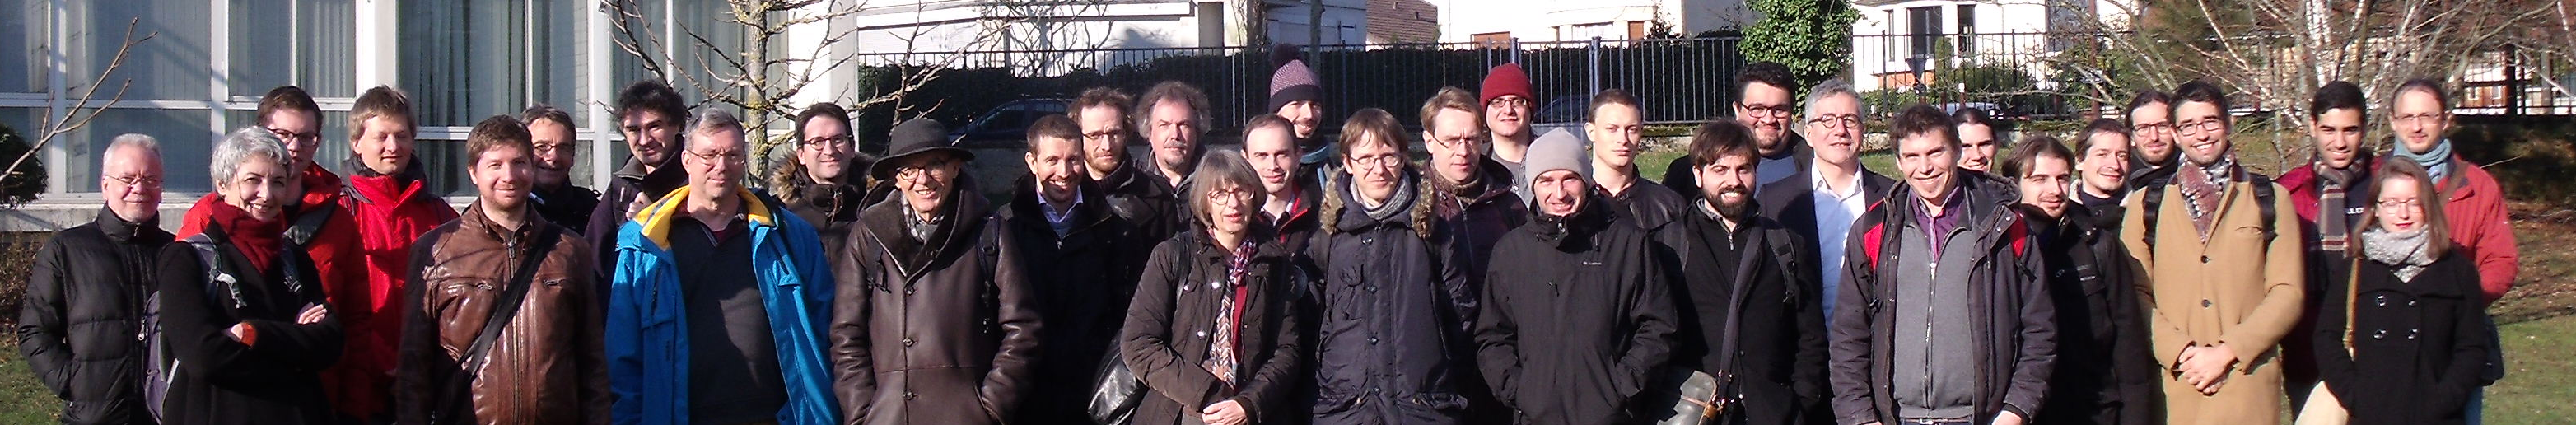
\includegraphics[height=2cm]{photo.png}
\end{center}
During this meeting, the idea of making this proof of concept a
European infrastructure emerged.  Since then, colleagues from Belgium,
Germany, Romania, Serbia, Sweden, and the United Kingdom, from
academia and industry, have expressed their interest in participating
in this effort.  These researchers and engineers are ready to
contribute to develop this encyclopedia, aiming at sharing proofs,
under a creative commons licence, making them searchable, accessible,
interoperable, and reusable.
\end{shaded}

%%%%%%%%%%%%%%%%%%%%%%%%%%%%%%%%%%%%%%%%%%%%%%%%%%%%%%%%%%%%%%%%%%%%%%%%%%%%%%
\begin{shaded}
\vspace*{-0.5cm}
\begin{center}
{\bf \Large How do proofs contribute to safety and security of software?}
\end{center}

Imagine the following casino game. At the beginning, a player is given
eleven euros. At each round, she throws a six-sided dice. If the
results is a six, then the game ends.  If it is a five, a four, a
three, or a two, she is given twice the amount of money she already
has. If it is a one she loses two euros, if she has at least two.
When the game ends, the player wins the money she got, except if she
has zero, in which case she loses one million euros.

This game can be modeled by the following programme:
\begin{center}
    \begin{minipage}{10cm}
\begin{verbatim}
n = 11
stay = True;
while stay:
    roll = random.randint(1,6)
    if roll == 6:
        stay = False
    else:
        if roll >= 2:
            n = n + 2 * n
        else:
            if (n >= 2):
                n = n - 2
print(n)
\end{verbatim}
    \end{minipage}
\end{center}

To be on the safe side, the player wants to be sure, before starting
playing, that she will never finish with zero.  And indeed, at all times
the content of the variable {\tt n} is an odd number,
thus it cannot be zero. {\bf This property ``nothing bad happens'' is
called the ``safety'' of this program.} This property is a
consequence of two simple theorems of arithmetic:
$$\forall x~(\mbox{\it odd}(x) \Rightarrow \mbox{\it odd}(x + 2 * x))$$
$$\forall x~(\mbox{\it odd}(x) \Rightarrow \mbox{\it odd}(x - 2))$$
meaning that, for all $x$, if $x$ is an odd number, then $x+2*x$ and $x-2$ are odd numbers too.
Hence, proving the safety of this programme amounts to prove these two
theorems.

Let's now consider the case where there is a tiny bug in the
program. For instance the {\tt 2} has been replaced by a {\tt 3} in
the instruction {\tt n = n + 2 * n}. The programme is then unsafe as
shown by the sequence $11, 9, 7, 5, 3, 1, 4, 2, 0$. Yet, testing this
program will, most likely, not reveal this bug, since it only
manifests very rarely.  In contrast, attempting to prove the
correctness of this program will reveal the bug as it is impossible to
prove the proposition
$$\forall x~(\mbox{\it odd}(x) \Rightarrow \mbox{\it odd}(x + 3 * x))$$
\end{shaded}

%%%%%%%%%%%%%%%%%%%%%%%%%%%%%%%%%%%%%%%%%%%%%%%%%%%%%%%%%%%%%%%%%%%%%%%%%%%%%%
%\begin{shaded}
%\vspace*{-0.5cm}
%\begin{center} {\bf \Large When mathematics are needed to verify the
%    correctness of a programme}
%\end{center}
%
%Prime numbers are used in a wide variety of applications:
%pseudo-random number generation, cryptographic algorithms, etc.  Thus,
%verifying the correctness of complex primality testing algorithms is
%critical.
%
%To do so, we need first to define primality, for instance
%
%$$prime(p) := 1<p \wedge (\forall n, (1<n\wedge n<p) \Rightarrow \neg(n\mid p))$$
%
%where $\wedge$ is the conjunction, $\Rightarrow$ is the implication,
%$\neg$ is the negation, and $n\mid p$ means that $n$ divides $p$.
%
%To lower the cost of primality testing, we use tests that are more
%efficient than the naive use of the definition.  For instance, a very
%simple improvement is to test the divisibility of the considered
%number, not by each of the smaller natural numbers, but only up to its
%square root.  Indeed, if a natural number $p$ can be factored into the
%product of two smaller natural numbers $m$ and $n$, one of them has to
%be smaller than or equal to the square root of $p$.  Therefore, one
%could give the following more complex, but more efficient, definition:
%
%$$prime'(p) := 1<p \wedge (\forall n, (1<n \wedge n*n\leq p) \Rightarrow \neg(n\mid p))$$
%
%To ensure that these definitions are equivalent one needs to prove
%the following statement:
%
%$$\forall p, prime'(p) \Leftrightarrow prime(p)$$
%
%It would have been easy to introduce a small bug
%in the new definition.  For example, one could have written
%$n*n < p$, instead of $n*n \leq p$.
%This would have resulted in accepting squares of primes as primes.
%
%Yet, attempting to prove the equivalence of these two definitions would
%have revealed the bug, as they cannot be proven to be equivalent.
%\end{shaded}

%%%%%%%%%%%%%%%%%%%%%%%%%%%%%%%%%%%%%%%%%%%%%%%%%%%%%%%%%%%%%%%%%%%%%%%%%%%%%%
\begin{shaded}
  \vspace*{-0.5cm}
  \begin{center}
    {\bf \Large What is a formal proof? What is a proof system?}
    \end{center}

Since Antiquity, we have known that
proofs, both purely mathematical ones, as in Euclid's elements or the
recent proof of the Kepler's conjecture by Thomas Hales, and proofs used
to establish the safety and security of software, can be built with a
limited number of rules, for example
\begin{itemize}
\item From $A\Rightarrow B$ (``$A$ implies $B$'') and $A$, deduce $B$.
\item From $A$, deduce $A\vee B$ (``$A$ or $B$'').
\item etc.
\end{itemize}
Yet for most of mathematical history, proofs have been written in
a pidgin of natural language and mathematical formulas. When proofs are
very long (as it is often the case for the proofs used in safety and security,
but also for some proofs in pure mathematics), mistakes are
very difficult to detect. For instance, dozens of wrong proofs of
the parallel postulate have been given through history, sometimes by the
best of mathematicians such as Ptolémée, Proclus, al-Haytam, Tacket,
Clairaut, Legendre, etc.

In the 1960s, Robin Milner and Nicolaas De Bruijn noticed that the
correctness of a mathematical proof could be checked by a
computer. This led to the development of the two first proof systems
in history: Milner's LCF and De Bruijn's Automath.

For instance, from the axioms
$$\forall x~(\mbox{\em philosopher}(x) \Rightarrow \mbox{\em human}(x))$$
$$\forall x~(\mbox{\em human}(x) \Rightarrow \mbox{\em mortal}(x))$$
we can deduce
$$\forall x~(\mbox{\em philosopher}(x) \Rightarrow \mbox{\em mortal}(x))$$
In the language implemented in Automath, this proof is written
$$\lambda x \lambda h~(g~x~(f~x~h))$$
\end{shaded}

%%%%%%%%%%%%%%%%%%%%%%%%%%%%%%%%%%%%%%%%%%%%%%%%%%%%%%%%%%%%%%%%%%%%%%%%%%%%%%
\begin{shaded}
\vspace*{-0.5cm}
  \begin{center}
{\bf \Large What is a theory?}
\end{center}

Deduction rules such as ``From $A \Rightarrow B$ and $A$, conclude
$B$'' are universal, but building proofs requires more rules, that are
often specific to a domain of knowledge and are called
``axioms''. Examples are the axioms of geometry, the axioms of
arithmetic, etc. These axioms constitute a theory.

At the beginning of the 20$^{\mbox{\footnotesize th}}$ century, an
axiomatic theory, {\em set theory}, has been proposed to express all
mathematical proofs. In the first half of the 20$^{\mbox{\footnotesize
    th}}$ century a few variants of set theory have been proposed, as
well as a few alternatives (such as \emph{Simple Type Theory}).  But
because these theories had not been designed for being implemented on
a computer, each proof system such as Coq, Isabelle/HOL, Mizar,
Atelier B, etc. implements its own theory.  {\bf Thus the rise of
computer-checked formal proofs has led to a multiplication of
alternative theories for mathematics.

This is the major obstacle to interoperability between proof systems.}
\end{shaded}

%%% Local Variables:
%%%   mode: latex
%%%   mode: flyspell
%%%   ispell-local-dictionary: "english"
%%% End:


\section{Objectives}

\begin{todo}{}\color{red}
  Describe the overall and specific objectives for the project1, which should be clear, measurable, realistic and achievable within the duration of the project. Objectives should be consistent with the expected exploitation and impact of the project (see section 2).
\end{todo}

\begin{figure}
\begin{framed}
  \begin{itemize}
\item[LIL 1:]
The theory implemented in the system has been defined in
the lambda-Pi-calculus modulo theory and in Dedukti.

\item[LIL 2:]
The system has been instrumented so some of its proofs can be exported
and checked in Dedukti.

\item[LIL 3:]
A significant part of the library of the system has been exported and checked in
Dedukti.

\item[LIL 4:]
A tool has been defined to analyze the Dedukti proofs for the system,
detect those that can be expressed in a theory weaker than that of the
system, and translate those proofs into a weaker logic.

\item[LIL 5:]
Certain proofs of the system have been made available in Logipedia.

\item[LIL 6:]
All proofs of the system have been exported, translated,
and made available in Logipedia.
\end{itemize}
\caption{The Logipedia integration levels (LIL)\label{lil}}
\end{framed}
\end{figure}

To foster the interoperability of proof systems and the sustainability
and the cross-verification of formal proofs, we propose to collect
them in an online encyclopedia, called {\sf Logipedia}.  For each
proof, {\sf Logipedia} will indicate in which systems it can be used
and, when this is the case, it will provide a version of this proof in
the theory of these systems.

Such a project will not only foster the use of formal proofs in
research in mathematics and computer science, but also in industry, by
allowing cross-verification, sustainability, and interoperability of
formal proofs, and in education, freeing the teaching of formal proof
technology from being bound to one system.

Such a project can only have a worldwide ambition. However, as a
majority of proof systems are developed in Europe, there is a unique
opportunity for Europe to take the lead on such a project and prepare
the grounds for the economic spinoffs from the project benefiting
European industry. That is why the consortium gathers most of the
European actors active on formal proof systems, while also developing
links with non-European partners.

Building this encyclopedia is {\em per se} a networking activity
between the partners, from academia and industry, involved in the
project.  Currently, we know how to express the theories of {\sf HOL
  Light} \cite{Assaf12}, {\sf Matita} \cite{Assaf15}, {\sf Coq} and
{\sf FoCaliZe} \cite{Cauderlier16} in {\sf Dedukti} and recheck proofs
developed in these systems.  We aim at including, in twenty years, all
formal proofs developed at that time.
In the next four years, we plan to address the theories of {\sf
  Abella}, {\sf Agda}, {\sf Atelier B}, {\sf HOL4}, {\sf Isabelle},
{\sf Minlog}, {\sf Mizar}, {\sf SMT-Lib}, \tlaplus, {\sf Why3}, {\sf
  LFSC}, {\sf PVS}, and {\sf TSTP}.  Other systems, such as {\sf
  ACL2}, {\sf IMPS}, {\sf Lean}, {\sf Nuprl}, and {\sf Rodin}, are
kept for later, except if some other partners join the project (Figure
\ref{systems}). This effort will require, and contribute, to build a
network of research teams, much stronger than what we currently have.

Beyond our main focus on interactive systems, we also plan to
integrate some proofs coming from automated theorem provers, SMT
solvers, and model checkers, when these proofs have a manageable
size. We already have experience with Archsat \cite{Bury19}, iProver
\cite{Burel10}, and Zenon \cite{CauderlierHalmagrand15}. We plan to go
further in this direction, in cooperation with our colleagues working
on LFSC \cite{Stump09}. Thus beyond the teams focused on formal proofs, we
will extend this network to teams of neighbour communities, such as
the automated theorem proving community and the SAT/SMT community.

To measure the level of integration of an existing proof system and
associated proof library in {\sf Logipedia}, we introduce a metric:
{\em the {\sf Logipedia} integration levels} (Figure \ref{lil}) that
counts six levels.  Among the 17 systems we shall focus on we plan to
increase the {\sf Logipedia} integration levels of 10 of them to level
5 or 6.

The various systems addressed in the project are currently at those levels:

\begin{tabular}{ll}
Matita:& level 5\\
FoCaliZe:& level 3\\
HOL Light:& level 5\\
Coq:& level 2\\
Agda:& level 2\\
Atelier B:& level 2\\
Isabelle:& level 2\\
HOL4:& level 1\\
TSTP:& level 1\\
Minlog:& level 0\\
PVS:& level 0\\
Abella:& level 0\\
Mizar:& level 0\\
TLA+:& level 0\\
SMT-Lib:& level 0\\
Why3:& level 0\\
LFSC:& level 0\\

\end{tabular}

and we plan to increase these levels to 

\begin{tabular}{ll}
Matita:& from level 5 to level 6\\
HOL Light:& from level 3 to level 5\\
FoCaliZe:& from level 3 to level 5\\
Coq:& from level 2 to level 5\\
Agda:& from level 2 to level 3\\
Atelier B:& from level 2 to level 5\\
Isabelle:& from level 2 to level 5\\
HOL4:& from level 1 to level 5\\
TSTP:& from level 1 to level ???\\
Minlog:& from level 0 to level 3\\
PVS:& from level 0 to level 2\\
Abella:& from level 0 to level 2\\
Mizar:& from level 0 to level 3\\
TLA+:& from level 0 to level 2\\
SMT-Lib:& from level 0 to level ???\\
Why3:& from level 0 to level ???\\
LFSC:& from level 0 to level ???\\

\end{tabular}

This encyclopedia will be freely accessible through a web browser,
from any country in Europe and beyond. But an important effort will be
made to make this encyclopedia accessible to a large community of
specialists and non-specialists, but structuring the contents on
libraries, books, chapters, etc. Some of the libraries we start with
already have a structure (modules, qualified names, etc.) that it is
important to preserve.

We shall also develop ergonomic interfaces, search engines, etc. 


Finally, this project will trigger joint research activities between
its users and between its developers.  First, there are several
theories for which we do not have yet reached level 1, and for which
we need to understand how to express then in {\sf Dedukti}. Which is
an obvious joint research activity. Then, we need to define algorithms
to eliminate some axioms from proofs. Many such algorithms already
exist to eliminate the excluded middle, the axiom of choice, or the universes
from a given proof. We need to develop new ones, more specific to the theories
we address in this project.

In addition, each library contains definitions of natural numbers,
real numbers, etc. and, most importantly, logical connectors, that
must be aligned, that is structural results proved for one definition
of real numbers must be transported to any definition of an isomorphic
structure.

All these objectives contribute to building a new formal proof
community, focused on the values of knowledge exchange and
sustainability.

%%% Local Variables:
%%%   mode: latex
%%%   mode: flyspell
%%%   ispell-local-dictionary: "english"
%%% End:



\section{Relation to the work program}

\begin{todo}{}\color{red}
  Indicate the work programme topic to which your proposal relates, and explain how your proposal addresses the specific challenge and scope of that topic, as set out in the work programme.
\end{todo}

\begin{longtable}{|p{0.2\textwidth}|p{0.75\textwidth}|}
\hline
{\bf Research \newline e-infrastructures for formal proofs}
&
Proof systems and automated theorem provers are research
infrastructures. Each proof system comes with its own library, and
these libraries are also part of the research infrastructure.  Currently
these infrastructures are small, distributed and disconnected.\\
&
\hspace{0.4cm}
Logipedia aims at building a large, worldwide infrastructure from the
small ones by integrating them.  The integration effort is substantial
because the proofs in the various libraries are expressed in different
theories, and because key definitions are formalized in a different
way.  But this integration effort is doable and contributes to the
challenge of bringing to European researchers and engineers effective and
convenient access to the best research infrastructures, in order to
foster further advances in knowledge and technology.\\
&
\hspace{0.4cm}
This idea to structure a networking activity around the construction
and the use of an infrastructure is relatively new in computer science
and mathematics. Moreover Logipedia is not an infrastructure of
computers, like Grid'5000 is, but mostly an infrastructure made of
data and of algorithms manipulating these data.  As Logipedia is an
e-infratructure, its budget structure is different from a material
infrastructure. A small part of the resources is used for computers,
and a large part of the budget is used to develop networking
activities, trans-national, virtual and ergonomic access, and joint
research activities.\\
\hline
{\bf A starting commu-}
&
This project has never been supported under FP7 or Horizon 2020 calls.\\
{\bf nity} &
\hspace{0.4cm} It mobilizes twenty nine research groups (twenty one in
academia and eight in industry), which is
almost all the groups working on formal proof technology in Europe.
The success of the project requires such a large network.  Indeed,
just like, according to Metcalfe's law, the effect of a network is
proportional to the square of the number of connected users, we can
postulate that the effect of an infrastructure, like Logipedia, is
proportional to the product of the number of proofs it contains and
the number of its potential users, each of them being proportional to
the number of theories it supports. So, such a project needs a
critical mass to succeed. This is also why we have developed a corona
surrounding the project, constituted of four clubs of users: 
a club of industrial users, a club of academic users, a club of users in 
education and a club of users in publishing.
These clubs
already have some members, but they will develop during the four years
of the project, preparing the long term future of the infrastructure.
The members of the club of industrial users have written letters 
explaining their interest in the project, that are in the appendix of this
document. {\color{red} Do not forget to include the letters.}
\\
&
\hspace{0.4cm}
These groups are located in eleven European countries.  Some of these
countries have a large number of participants, some others fewer,
reflecting the diversity of maturity of the research on formal methods
in Europe. This project will contribute to develop the formal proof
culture in the European countries where it is still inceptive.\\
&
\hspace{0.4cm}
We should also point out the originality of this project within the
European strategy of Research infrastructure.\\
&\\
&
$\blacktriangleright$ A novelty of this project is that is
investigates how infrastructures can be used in mathematics and in
computer science.\\
&\\
&
$\blacktriangleright$ It investigates how immaterial infrastructure
can be used to structure a research community, just like material ones
do.\\
&\\
&
$\blacktriangleright$ It is focused on mathematical {\em a priori}
knowledge, while most infrastructures are focused on {\em a
  posteriori} knowledge, issued from measures, observations,
experiments, and field surveys.\\
&\\
&
$\blacktriangleright$ It also investigates how a common infrastructure
articulates the relation between research and industry.
\\
\hline
{\bf Compliance policy with EU regulations}
&
A data management plan will be provided according to Inria’s
compliance policy with EU regulations. We also engage ourselves to
make the evolution of the Logipedia e-infrastructure compliant
with the European charter for access to research infrastructures.\\

\hline
{\bf Networking activities, trans-national access, joint re-}
&
Three work packages described below are dedicated to networking activities
to collect the data that constitute the infrastructure: the formal proofs
that constitute Logipedia.
\\
{\bf search activities}
&
\hspace{0.4cm}
Logipedia will be publicly and freely accessible online through any
web browser and trough a package management tool, so trans-national
and virtual access are provided directly. Its administration will be
decentralized in various places in Europe with two mirror sites in
Saclay and in München. But we go beyond trans-national and virtual
access.  Two work packages described below are dedicated to improving
the quality of the access to the encyclopedia.\\
&
\hspace{0.4cm}
Finally, this project fosters new joint research activities. First,
between the members of the consortium. Then, between the members of
the consortium and other academic partners, in particular those
developing automated theorem proving systems. Next, between the
consortium and the industrial users of proof systems. Finally, between
the industrial users themselves, as using proofs developed by others
will foster joint developments. Two more work packages are dedicated
to these research activities.  Such joint research activities
currently exist in Europe to some extent.  Such a joint project is a
unique opportunity to strengthen the existing ones and create new
ones.
\\
\hline
{\bf Towards standardization}
&
This project will be a stepping stone for a possible standardization
of proof languages.
\\
&
\hspace{0.4cm}
Unlike other communities in computer science, the formal proof
community is somewhat skeptical with respect to standardization. And
indeed, it would not make sense to standardize a theory for proof
systems, just like it would make no sense to propose Euclidean
geometry as a standard all geometers should use.  Instead, such a
cooperative effort can lead to the standardization of a logical
framework, that is a language to express theories and proofs in any of
these theories. Proceeding slowly and in a cooperative thus may change
the attitude towards standardization in the formal proof community and
make a standardization process more widely accepted.
\\
\hline
{\bf Inter-disciplinarity}
&
This project includes mathematicians, logicians, and computer
scientists and therefore is clearly inter-disciplinary.\\
&
\hspace{0.4cm}
Yet, Logipedia is inter-disciplinary in an even more fundamental
way. Proving properties of a piece of software driving a car or
piloting an aircraft require to formalize part of the physical world
in which this piece of software evolves. In the same way proving
properties of simulation software, requires to formalize some
properties of the simulated object.  Thus, just like mathematics and
software are involved in any part of modern science, formal proof will
eventually spread, over time, in all areas of science.\\
&
\hspace{0.4cm}
One major obstacle to the formalization of, for example, simulations
is that they typically depend on large bodies of knowledge in
mathematics and physics.  Different proof systems may be better
suited for different applications, thus there is a natural tendency
for a diversity of proof formats, just like there is a natural
tendency for diversity in the use of programming languages.  Yet, when
it comes to formalizing a particular physical simulation, one needs to
have all the necessary knowledge accessible from a single infrastructure.\\
&
\hspace{0.4cm}
Formal proofs will eventually become pervasive, and
different disciplines may be tempted to use different systems.
Because inter-disciplinarity is required to formalize physical world
simulations, a unifying language such as Logipedia for exchanging
formal proofs between theorem provers is a must-have.\\
\hline
\end{longtable}


%%% Local Variables:
%%%   mode: latex
%%%   mode: flyspell
%%%   ispell-local-dictionary: "english"
%%% End:


\section{Concept and methodology}

\begin{todo}{Concept}\color{red}
Describe and explain the overall concept underpinning the project. Describe the main ideas, models or assumptions involved. Identify any inter-disciplinary considerations and, where relevant, use of stakeholder knowledge. Where relevant, include measures taken for public/societal engagement on issues related to the project;
  
Describe how the participating Research Infrastructures will be integrated to provide, at European and, where relevant, global level, an overarching Research Infrastructure service, contributing to structuring the European Research Area, and, where relevant, global cooperation on Research Infrastructures. Describe also how this ensemble will ensure complementarity and coherence with the existing European Research Infrastructures landscape, including ESFRI infrastructures and existing integrating activities for advanced communities;

Describe any national or international research and innovation activities which will be linked with the project, especially where the outputs from these will feed into the project;
\end{todo}

\begin{todo}{Methodology}\color{red}
  Describe and explain the overall methodology, distinguishing, as appropriate, activities indicated in the relevant section of the work programme. Describe in particular how the various types of activities (i.e. networking activities, trans-national and/or virtual access activities, and joint research activities) will form a coherent and coordinated set of components contributing to the same objectives.

  Where relevant, describe how the gender dimension, i.e. sex and/or gender analysis is taken into account in the project’s content.
  Please note that this question does not refer to gender balance in the teams in charge of carrying out the project but to the content of the planned research and innovation activities . Sex and gender analysis refers to biological characteristics and social/cultural factors respectively. For guidance on methods of sex / gender analysis and the issues to be taken into account, please refer to \url{http://ec.europa.eu/research/swafs/gendered-innovations/index_en.cfm?pg=home} 
\end{todo}

{\bf \Large (a) Concept}

\begin{framed}
\begin{center}
{\bf \Large How do proofs contribute to safety and security of software?}
\end{center}
  
Imagine the following casino game. At the beginning, a player is given
eleven euros. At each round, she throws a dice. If the results is a
six, then game is over.  If it is a five, a four, a three, or a two,
she is given twice the amount of money she already has. If it is a one
she is taken two euros, if she has at least two.  When the game is
over, the player wins the money she got, except if she has zero, in
which case she looses one million.

This game can be modeled by program $p$
%import random 
\begin{verbatim}
n = 11
stay = True;
while stay: 
    roll = random.randint(1,6)
    if roll == 6:
        stay = False
    else:
        if roll >= 2:
            n = n + 2 * n
        else:
            if (n >= 2):
                n = n - 2
print(n)
\end{verbatim}

To be on the safe side, the player wants to be sure, before starting
playing, that she will never finish with zero.  And indeed, in all runs,
the content of the variable {\tt n} is always an odd number, thus it
cannot be zero. This property is a consequence of two simple
theorems of arithmetic
$$\forall x~(\mbox{\it odd}(x) \Rightarrow \mbox{\it odd}(x + 2 * x))$$
$$\forall x~(\mbox{\it odd}(x) \Rightarrow \mbox{\it odd}(x - 2))$$
%$$\forall x~(\mbox{\it odd}(x) \Rightarrow \mbox{\it odd}(x))$$
Hence, verifying the safety of this program, that is that the
proposition 
${\mbox{\it safe}}(p)$ holds, 
amounts to prove these three theorems of arithmetic.

A tiny bug in the program, for instance replacing the {\tt 2} by a
{\tt 3} in the the line {\tt n = n + 2 * n} makes the program unsafe
as shown by the sequence $11, 9, 7, 5, 3, 1, 4, 2, 0$. Yet, testing
this program will, most likely, not reveal this bug, that manifests
very rarely.  In contrast, attempting to prove the correctness of this
program will
reveal the bug as it is impossible to prove the proposition
$$\forall x~(\mbox{\it odd}(x) \Rightarrow \mbox{\it odd}(x + 3 * x))$$
\end{framed}
\pagebreak
\begin{framed}
  \begin{center}
    {\bf \Large What is a formal proof? What is a proof system?}
    \end{center}
        
Since Antiquity, we have known that
proofs, both purely mathematical ones, as in Euclid's elements or the
recent proof of the Kepler conjecture by Thomas Hales, and proofs used
to establish the safety and security of software, can be built with a
limited number of rules, for example
\begin{itemize}
\item From $A \Rightarrow B$ and $A$, deduce $B$.
\item From $A$, deduce $A~\mbox{\it or}~B$.
\item ...
\end{itemize}
Yet, through history, most mathematical proofs have been written in
pidgin of natural language and mathematical formulas. When proofs are
very long (as it is often of the proofs used in safety and security,
but also of some proofs in pure mathematics), mistakes in proofs are
very difficult to detect. For instance dozen of wrong proofs of
parallel postulate have been given through history, sometimes by the
best mathematicians such as Ptolémée, Proclus, al-Haytam, Tacket,
Clairaut, Legendre...

In the 1960s, Robin Milner and Nicolaas De Bruijn noticed that the
correctness of a mathematical proof could be checked by a
computer. This led to the development of the two first proof systems
in history: Milner's LCF or De Bruijn's Automath.  From
the axioms
$$\forall x~(\mbox{\em philosopher}(x) \Rightarrow \mbox{\em human}(x))$$
$$\forall x~(\mbox{\em human}(x) \Rightarrow \mbox{\em mortal}(x))$$
we can deduce
$$\forall x~(\mbox{\em philosopher}(x) \Rightarrow \mbox{\em mortal}(x))$$
In the language implemented in Automath, this proof is written
$$\lambda x \lambda h~(g~x~(f~x~h))$$
\end{framed}

\begin{framed}
\begin{center}
{\bf \Large What is a theory?}
\end{center}

Deduction rules such as ``From $A \Rightarrow B$ and $A$, conclude
$B$'' are universal, but building proofs require more rules, that are
often specific to a domain of knowledge and are called
``axiom''. Examples are the axioms of geometry, the axioms or
arithmetic. These axioms constitute a theory.

At the beginning of the 20th century an axiomatic theory, {\em set
  theory}, has been proposed to express all mathematical proofs. In
the first half of the 20th century a few variants of set theory, and a
few alternatives have been proposed (such as Simple type theory).
But, because these theories had not been designed for being
implemented on a computer, the rise of computer checked formal proofs
has led to a multiplication of such alternative theories. Each proof system,
such as Coq, Isabelle/HOL, Mizar, Atelier B,
etc. implements its own theory.

This is the major obstacle to interoperability.
\end{framed}

\bigskip

\noindent
{\bf \Large Logical Frameworks}

We had, in the past, an (informal) proof of Pythagoras’ theorem
or Fermat’s little theorem. The same proof now has different
formalizations in PVS, Isabelle/HOL, Coq, etc., jeoprardizing the
universality of logical truth.

In the 19th century, the universality of logical truth has been
jeopardized in a similar way, by non-Euclidean geometries, as some
statements could be true in one geometry, but false in others.  But,
at the beginning of the 20th century, a solution was found.  The
definition of the various geometries in predicate logic
\cite{HilbertAckermann} restored the universality of logical truth,
allowing to determine which axiom was used in which proof and which
theorem held in which geometry.

Predicate logic is not a theory in itself, but it is a framework in
which one can express theories, as sets of axioms: {\em a logical
  framework}.  Expressing the various geometries in predicate logic
allowed to analyze which proof contained which axiom, and hence which
proof could be expressed in which theory.

In 1928, predicate logic was a huge success, since three important
theories used at that time (geometry, arithmetic and set theory) could
be expressed in it. But it also has limitations, which explains that
another of the major theories used at that time (Russell's type
theory, from The Principia Mathematica) has not been expressed in
it. Since then, several other theories, such as Church's type theory
\cite{Church40}, Martin-L\"of's type Theory \cite{Martin-Lof84}, and
the Calculus of constructions \cite{CoquandHuet88}, have also been
defined as autonomous theories. These theories are those implemented
in most of the current proof systems, yet they cannot be expressed in
predicate logic.

This failure has led, in the field of proof systems, to the
abandonment of predicate logic, and even of the concept of logical
framework: the theories implemented in Coq, Matita, HOL Light,
etc. are often defined as autonomous systems, and not in a logical
framework.

However, a different line of research has attempted to understand the
limitations of predicate logic and to propose other logical frameworks
repairing them. The most prominent limitations of predicate logic are
the lack of function symbols binding variables, the lack of a syntax
for proof terms, the lack of a notion of computation, the lack of a
notion of cut for axiomatic theories, and the impossibility to express
constructive proofs. These limitations have led to the development of
logical frameworks such as $\lambda$-Prolog \cite{NadathurMiller88,
  MillerNadathur12}, Isabelle \cite{Paulson90}, the $\lambda
\Pi$-calculus (also called the ``Edinburgh logical framework'')
\cite{HarperHonsellPlotkin91}, Deduction modulo theory
\cite{DowekHardinKirchner03, DowekWerner03}, Pure Type Systems
\cite{Berardi88,Terlouw89}, and ecumenical logics
\cite{Prawitz15,Dowek15,PereiraRodriguez17}.

All these logical frameworks have been unified in the $\lambda
\Pi$-calculus modulo theory \cite{CousineauDowek07}, implemented in
the system Dedukti \cite{Assaf16}
on which Logipedia is based. Geometry, arithmetic and set
theory, but also Russell's type theory, Church's type theory,
Martin-L\"of's type theory, and the Calculus of constructions can be
expressed in this framework.

For instance, although the details are not important, Church's type
theory can be expressed in Dedukti , with 8 déclarations and 3
rewrite rules.
\begin{framed}
$\begin{array}{rcl}
type&:&Type\\
\eta&:&type \rightarrow Type\\
o&:&type\\
\mbox{\it nat}&:&type\\
\mbox{\it arrow}&:&type \rightarrow type \rightarrow type\\
\varepsilon&:&(\eta~o) \rightarrow Type\\
\Rightarrow&:&(\eta~o) \rightarrow (\eta~o) \rightarrow (\eta~o)\\
\forall&:&\Pi a:type~(((\eta~a) \rightarrow (\eta~o)) \rightarrow (\eta~o))\\
\\
(\eta~(\mbox{\it arrow}~x~y)) &\longrightarrow& (\eta~x) \rightarrow (\eta~y)\\
(\varepsilon~(\Rightarrow~x~y)) &\longrightarrow& (\varepsilon~x) \rightarrow (\
\varepsilon~y)\\
(\varepsilon~(\forall~x~y)) &\longrightarrow& \Pi z:(\eta~x)~(\varepsilon~(y~z))
\end{array}$
\end{framed}

So the theories implemented in various systems can all be expressed in
Dedukti and the proofs developed in these systems can be translated to
Dedukti. Just like in the case of non Euclidean geometry, this allows
to analyse the symbols and rewrite rules used in each proof
\cite{Thire18,Dowek17} (a domain traditionally called ``reverse
mathematics'' \cite{Friedman76,Simpson09}) and to deduce in which
systems each proof can be used.  This analysis is the basis of the
interoperability between proof systems.


\bigskip

\noindent
{\bf \Large The Logipedia integration levels}

\medskip

Thus, to make a formal proof, developed in some system $X$, accessible to
the users of other systems, the first step is to express the theory
$D[X]$, implemented in the system $X$, in the logical framework
  Dedukti.  Then, we must instrument the system $X$ so that the proof
can be exported from it, as a piece of data, expressed as a proof in
$D[X]$ and included in Logipedia. Next, we need to analyze this
proof in order to determine which symbols, axioms and rewrite rules of
$D[X]$ it actually uses and, thus, in which alternative theories it
can be expressed.  Finally, we must align its concepts with the
definitions already present in Logipedia and decide where it
fits in the general structure of the encyclopedia.

To measure the level of integration of an existing proof system and
associated proof library in Logipedia, we introduce a metric:
{\em the Logipedia integration levels} (Figure \ref{lil}) that
counts six levels.  

\begin{framed}
\begin{center}
{\bf The Logipedia integration levels (LIL)\label{lil}}
\end{center}

\begin{itemize}
\item[LIL 1:]
The theory implemented in the system has been defined in
the $\lambda\Pi$-calculus modulo theory and in Dedukti.

\item[LIL 2:]
The system has been instrumented so some of its proofs can be exported
and checked in Dedukti.

\item[LIL 3:] A significant part of the library of the system has been
  exported and checked in Dedukti.

\item[LIL 4:] A significant part of the library of the system have
  been made available in Logipedia.

\item[LIL 5:]
A tool has been defined to analyze the Dedukti proofs for the system,
detect those that can be expressed in a theory weaker than that of the
system, and translate those proofs into a weaker logic.

\item[LIL 6:]
All proofs of the system have been exported, translated,
and made available in Logipedia.
\end{itemize}
\end{framed}

The sixteen systems addressed in this project currently have different
integration levels, and we have different targeted levels for them.. 

\begin{center}
\begin{tabular}{|l|c|c|}
\hline
System & current level & targeted level\\
\hline
Matita & 5 & 6\\
\hline
HOL Light & 3 & 5\\
\hline
FoCaLiZe & 3 & 5\\
\hline
Coq & 3 & 5\\
\hline
Agda & 2 & 4\\
\hline
Atelier B & 1 & 5\\
\hline
ProB & 1 & 5\\
\hline
Isabelle & 2 & 5\\
\hline
HOL4 & 1 & 5\\
\hline
TSTP & 1 & {\color{red} ???}\\
\hline
Minlog & 0 & 4\\
\hline
PVS & 0 & 2\\
\hline
Abella & 0 & 2\\
\hline
Mizar & 0 & 4\\
\hline
Smart & 0 & 3\\
\hline
TLA+ & 0 & 2\\
\hline
 Why3 & 0 & {\color{red} ???}\\
\hline
LFSC & 0 & {\color{red} ???}\\
\hline
\end{tabular}
\end{center}

These systems can be roughly divided into two groups. Those in the
first half of the array (Matita, HOL Light, 
  FoCaLize, Coq, Agda, Atelier B, ProB, Isabelle,
HOL4, and TSTP) for which we have preliminary results and
that we plan to bring to a very high level of integration. Those in
the second half (Minlog, PVS, Abella, Mizar,
Smart, TLA+, SMT-Lib, Why3, and LFSC) with which we
are starting and for which our goal are less ambitious.

These two groups of systems will be addressed in different
work packages, but both are key to the project. The first ones will
constitute Logipedia in 2024 and the second ones prepare the
long term future of the infrastructure.

\bigskip

\noindent
{\bf \Large Instrumentation}

\medskip

Consider a system $X$ at LIL 1, so the basic theory $D[X]$ has
already been expressed in Dedukti. The next step is to implement a
method to automatically translate proofs from system $X$ to its
expression in Dedukti, and make these proofs available in Logipedia so
they can be exported to other systems. This step is called the
\emph{instrumentation} of system $X$.

The systems considered in this project fall into three broad classes:
\begin{description}

  \item[Systems based on dependent type theory.] Agda, Coq, and Matita
  are theorem provers based on Martin-L\"of's intuitionistic type
  theory.

  \begin{itemize}
    \item Coq is an interactive theorem prover developed at Inria
    since the 1984.  It is based on Type Theory and was used to
    formally verify the correctness of both industrially relevant
    software such as the CompCert C compiler and complex mathematical
    proofs such as the one of the Four Color theorem and the one of
    the Odd Order theorem. In 2013 Coq received the ACM system award.

    \item Matita is an interactive theorem prover developed at the
    University of Bologna and used for teaching logic courses and to
    verify software and mathematical proofs, with special attention to
    predicative foundations. The first generation of the system (up to
    version 0.5.9) was born as a by-product of the MoWGLI FET-Open
    Project, it was compatible with the logic of Coq and it could
    re-use its libraries. It was an important test-bench for the
    integration of Mathematical Knowledge Management techniques with
    Interactive Theorem Proving, featuring for example a library of
    theorems distributed over multiple servers, innovative indexing
    and search techniques and automatic translation of proofs between
    declarative and procedural styles. The second generation of the
    system (up to the current version 0.99.3) was a re-implementation
    from scratch that departed from the logic of Coq and that
    experimented with the most concise ways to implement an efficient
    theorem prover. Several ideas later migrated into Coq. The
    currently available largest library is the formal certification of
    a complexity-preserving and cost-model-inducing compiler from C to
    MCS-51 machine code, developed in the FET project CerCo (Certified
    Complexity).

    \item Agda is a dependently typed programming language and
    interactive proof assistant developed at Chalmers University of
    Technology as well as other places in Europe. The theory of Agda
    is similar to Coq and Matita, but is more focused on interactive
    development and direct manipulation of proof terms (in contrast to
    using a tactic language to generate the proof terms). To support
    the construction of proof terms, Agda provides powerful features
    such as dependent pattern and copattern matching, eta equality for
    functions and record types, first-class universe polymorphism, and
    definitional proof irrelevance. In addition, Agda provides an
    experimental option for extending the language with user-defined
    rewrite rules, which are very similar to the rewrite rules
    provided by Dedukti.
  \end{itemize}

  \item[Systems based on simple type theory.] (HOL4, Isabelle)
  \ednote{We still need some text to go here!}

  The HOL4 proof assistant is home to a few medium to large scale
  specifications and associated proof developments that have value
  outside of HOL4. These specifications include the formal semantics
  of the CakeML language (and its verified compiler) and an extensive
  specification of the ARM instruction set architecture (ISA) as
  formalised by Anthony Fox at the University of Cambridge.

  Isabelle as a logical framework \cite{paulson700} is an intermediate
  between Type-Theory provers (like Coq or Agda) and classic LCF-style
  systems (like HOL Light or HOL4).

\item[Systems based on set theory and first-order logic.] Atelier B,
  Rodin and ProB are platforms or tools to develop models written
  using the B method, a version of set theory expressed in predicate
  logic.  A model in these systems encodes a state machine constrained
  by invariant properties. Verification of the model correctness
  implies to verify some proof obligations produced by a weakest
  precondition calculus. For example, spanning trees algorithms,
  distributed algorithms, access control policies have been formalized
  respectivement in EventB and B method.

  The development process for the B method is based on formal proof:
  proof obligations are automatically generated and must be proven by
  automatic or interactive provers. This can include external solvers
  such as SMT solvers, and (in the case of ProB) constraint solvers
  such as Sicstus Prolog. The difference between Atelier B and Rodin
  lies mainly in the refinement process they implement: in the B
  method used by Atelier B refinement is done by deriving a program,
  while in Event-B used by Rodin refinement is done by defining a
  model of the system and iteratively introducing details. Finally,
  ProB is an animator and model checker: it helps users to gain
  confidence in their specifications, and it can be used as a
  disprover to discover counter-examples to proof obaligations.

  Smart is based on a classical first-order logic extended with rank-1
  polymorphism, algebraic datatypes, recursive definitions and
  inductive predicates. ProvenTools will turn models implemented in
  Smart to proof obligations which can be proved in the system using a
  mix of interactive and automated proving. The resulting proofs are
  reviewable objects, akin to proof traces built of the various atomic
  proof rules supported by ProvenTools' kernel, such as definition
  unfolding, case analysis or equality propagation.
\end{description}
Despite the large differences between these three classes of provers,
there are several common points between them where solutions that work
for one system can also be applied to other systems.
%
Concretely, we plan to tackle the following
research challenges:
\begin{description}

\item[Improving encodings.] Since Dedukti is designed to be a small
  logical framework with a minimal number of features, there are many
  features in the systems we consider that are not supported in
  Dedukti. Instead, such features need to be encoded in some way. In
  this work package, we consider systems for which it is known how to
  encode all features \emph{in theory}. However, depending on the
  choice of encoding, the instrumentation may be very hard or even
  unfeasible in practice. For example:
  \begin{itemize}

    \item Many Agda libraries (as well as some Coq libraries) rely
    heavily on type-directed conversion rules such as eta-equality for
    functions and record types, or definitional proof
    irrelevance. Dedukti does not provide type-directed conversion
    directly, so instead these rules have to be encoded by adding
    additional type information to the proof terms. This can hence
    lead to a large blow-up in the size of those proof terms, and thus
    greatly increase the cost of typechecking.

    \item Coq, Agda, and Matita all provide support for coinductive
    (infinite) structures, which are not supported natively in
    Dedukti. These structures can be encoded by rewrite rules in
    Dedukti, but this may cause the typechecker to go into an infinite
    loop.

    \item A few of the systems rely on AC rewriting (i.e.~rewriting
    modulo associativity and commutativity of certain operations), for
    example to encode universe polymorphism in dependent type
    theories. While Dedukti has support for AC rewriting, the current
    implementation is very slow, which makes typechecking the proofs
    in Dedukti unfeasible.

  \end{itemize}
  Finding better ways to encode such features could have a great
  impact on the quality and speed of the translation process.  We plan
  to investigate two possible approaches to improve the encodings of
  common features of proof assistants in Dedukti. First, we will
  investigate whether some information in the current encodings is
  redundant and can thus be omitted. Second, if this is not possible
  we will investigate what minimal changes need to be made to Dedukti
  itself in order to overcome these limitations.

  \item[Reconstructing transient proof components.] In all theorem
  provers, there is some information that is created during the
  process of checking a proof that is not stored in the final proof
  term. In systems such as Coq, Agda, and Matita, this concerns for
  example the types of each subexpression. In other systems such as
  HOL4, Isabelle, Atelier B, and Rodin, even more information about
  the proof is discarded and only the high-level proof steps remain.
  However, the translation from the system to Dedukti might rely on
  this transient information. Developing a method to reconstruct this
  transient information is thus crucial to the goals of this work
  package.

  In order to instrument systems with transient proof information, the
  proof terms need to be complemented with this transient information
  by either logging or re-synthesizing it on demand. Both approaches
  may be used, depending on the the tradeoff between computation time
  and space for storage.

  However, this approach is insufficent for systems that rely on
  external provers such as Isabelle or Event B. In order to handle
  these cases, we will instrument these external provers so they can
  produce the missing parts of the proof terms. 

  \item[Producing more compact proofs.] When translating a proof from
  some system $X$ to Dedukti, we want to produce proof terms that are
  as small as possible, so it is easy to store them, recheck them, or
  export them to a different system. However, there are at least two
  reasons why proof terms might become large. First, a typical proof
  in system $X$ might be very large (because big parts of it are
  constructed automatically). Second, translating a proof from $X$ to
  its encoding in Dedukti might greatly increase the size of the
  proof, for example by normalizing it or by adding type annotations.
  This means translating the proofs can take a very long time, and
  doing anything with the translated proof will be difficult. This
  also has an obvious impact on the exporting of complete libraries to
  Dedukti, which is the goal of WP3.

  To reduce the size of proof terms produced by the translation to
  Dedukti, we plan to investigate how to avoid unneccessary
  normalization or duplication of (parts of) proofs. We will also
  investigate what parts of each proof can be safely omitted because
  they can be inferred from the rest of the proof.
\end{description}

For each of the systems considered in this work package, we can
identify some preliminary work on translating proofs to Dedukti. Some
of these tools are in a preliminary stage and can only handle toy
examples, while others have been used to export whole libraries but
have not been updated to work with the latest version of the
system. Concretely, we plan to build upon the previous work done on
the following tools:
\begin{itemize}
\item The standard and arithmetic libraries of Matita has been the
  first libraries to be exported to Logipedia using Krajono, a fork of
  Matita. The forked system is also actually the only one able to
  import Logipedia proofs. The choice of Matita as a test-bench for
  Logipedia is easily understood considering that the implementation
  of the 0.99.x series was aimed at obtaining a well-documented,
  minimal but fast implementation of a theorem prover, two order of
  magnitudes smaller than Coq.  We plan to make this translation a
  part of the code of Matita itself so that it is maintained with the
  rest of the system.
\item CoqInE is a prototype tool that can translate Coq proofs to
  Dedukti. Recent work to include advanced features of Coq, such as
  universe polymorphism, has dramaticaly increased the coverage of
  this translation. We plan to make this translation a part of the
  code of Coq itself so that it is maintained with the rest of the
  system.
  \item In the summer of 2019, Guillaume Genestier worked together
  with Jesper Cockx on the implementation of an experimental
  translator from Agda to Dedukti during a research visit at Chalmers
  University in Sweden. This translator is still work in progress, but
  it is already able to translate 142 modules of the Agda standard
  library (about 25\%) to a form that can be checked in Dedukti. This
  exploratory work uncovered several challenges and opportunities for
  further work (see research challenges above).
  \item The inference kernel of Isabelle has already been instrumented
  to output proofs as $\lambda$-terms that can be understood by
  Dedukti. However, this has so far been only used for small examples
  \cite{Berghofer-Nipkow:2000:TPHOL}. The challenge is to make
  Isabelle proof terms work robustly for the basic libraries and
  reasonably big applications.  Preliminary work by Wenzel (2019) has
  demonstrated the feasibility for relatively small parts of
  Isabelle/HOL, but this requires scaling up.
  \item HOL4 has support for exporting proofs to the OpenTheory proof
  exchange format, and there has been some work on importing
  OpenTheory proofs into Dedukti.
  \item In the context of the BWare project, an encoding of the set
  theory of the B method has been provided as a theory modulo, i.e. a
  rewrite system rather than a set of axioms. This encoding is used by
  the automatic prover Zenon modulo which features a backend to
  Dedukti. Thus, as a first step through instrumentation of Atelier B
  and Rodin, proof obligations coming from Atelier B can be proved by
  Zenon modulo producing Dedukti proofs, hence providing a better
  confidence in the proofs produced by the native proof tools of
  Atelier B \cite{Bware}.
\end{itemize}

\bigskip
\noindent
{\bf \Large Automatic theorem provers: SAT/SMT solvers, first-order provers, etc.}

\medskip

We have discussed, in the last section, the instrumentation of proof
systems, that is interactive systems, where the users build formal
proofs with the help of the machine. Automatic Theorem Proving are
another type of systems, where the machine build proofs without any
human intervention. The proofs built by these systems are often
expressed in simpler theories than those developed using proof
systems, but they are not of a different nature. We will also include
in Logipedia proofs built by such automatic systems, whether they are
called automatic theorem provers, SAT solvers, SMT solvers, etc.

Several reasons explain the importance of these proofs for Logipedia.
{\em Per se}, many formal proofs nowadays rely on the use of automatic
provers. They cover various domains and various kinds of application,
{\em e.g.} combinatorial
mathematics~\cite{DBLP:journals/ai/KonevL15,DBLP:conf/sat/HeuleKM16},
where they are expected to solve one large propositional problem, or
proof of
programs~\cite{DBLP:conf/esop/FilliatreP13,DBLP:journals/pacmpl/ProtzenkoZRRWBD17},
where they are given thousands of small problems in a combination of
quantified theories.

In a complementary way, automatic theorem provers will be used to automatically make a
coherent whole out of Logipedia. A fruitful interaction between
formal proofs requires low-level glue which falls in the scope of automatic theorem provers.
For instance, they will be employed to fill the holes that appear when
considering provers with various granularity, to reduce the gaps between
proof systems, and to discharge proofs of concept alignment (in close
interaction with the work package 6).

Finally, automatic theorem provers will also benefit from
Logipedia. Obviously, Logipedia will be an extensive library of formal
statements that can be used and combined by automatic theorem provers
in their proof search. This is not trivial though: lemma selection is
crucial to avoid an overhead. It can also be a source of benchmarks to
evaluate their expressivity and automation.  Lastly, Logipedia and
Dedukti will form a framework to make automatic theorem provers
cooperate with each other and with other tools, in a safe way.

PF: TODO: Talk somewhere above about the various automatic theorem
proving tools, their specificity and why they are each of them useful
or would benefit from Logipedia

\medskip

\noindent
{\bf \large From automatic theorem provers to Dedukti}

Similarly to Interactive Theorem Provers, connecting ATPs to the Logipedia
infrastructure strongly relies on the ability for ATPs to import statements from
{\sf Dedukti} and export proofs in some theory in {\sf Dedukti}.

\begin{description}
\item[Instrumenting ATPs to produce proof traces.] The first step for connecting ATPs to the Logipedia infrastructure, and the library of proofs, is that ATPs should actually output some kind of proof, without enforcing strong requirement on the format or even the level of granularity of those proofs.  SAT (Satisfiability) solvers for propositional logic do have a perfectly well specified format for proof traces~\cite{TODO} and most SAT solvers are actually able to produce proof traces in that format.  So, considering SAT solvers, the current status is actually meeting the Logipedia needs on this aspect.

  Considering other automated reasoners however, it is mandatory to significantly improve the picture.  Some SMT (Satisifiability Modulo Theories) solvers do produce some kind of proof trace, but the format is specific to the solver, and the proofs are sometimes difficult to replay due to their granularity.  Most mainstream first-order theorem provers output proofs in a standardized language~\cite{TODO}, but this language does not clearly specify the semantics of the proof steps.  Model-checkers do not provide proof traces per se, although such traces would be useful for various usages and notably certification.

  Our goals are to improve reasoning tools to demonstrate the feasibility to
  produce sufficiently detailed proofs for connecting to Logipedia, and to
  design a set of theoretical methods and practical tools that can be used to
  further connect Logipedia to the other existing automated reasoners of the
  same kind.  We will work on three SMT solvers (alt-ergo, CVC4, veriT), two
  first-order provers (the E-prover, Zipperposition), and one model-checker
  (cubicle).  We will also consider more specific reasoning tools, with the aim
  to demonstrate that this approach also applies to more specific reasoners.  We
  envision to experiment the approach on a Coherent Logic reasoner.  These
  reasoners are particularly useful for geometry reasoning, and as such, they
  are quite complementary to the other considered automatic reasoners.  They are
  also very suitable as as a first experiment, since their proofs are fairly
  straightforward to interpret.  They thus constitute a very interesting low
  hanging fruit.
  
  It is not possible, and not even desirable, to require all tools to directly
  talk in the language of Logipedia.  Indeed, proof trace languages that are
  specific to one kind of reasoning tool are more appropriate than Dedukti for
  instrumenting already large pieces of software, enabling quick output, and
  allowing proof post-processing at the right level of abstraction on the
  produced proof traces.  Furthermore, provided that those proofs are detailed
  enough, translation of traces to Dedukti will not be a difficult task, and a
  the work necessary to translate proof traces for a myriad of very different
  reasoners will be implemented in a unique tool (Ekstrakto, see below) to take
  advantage of the fact that reasoning techniques, and thus proof methods, are
  themselves pretty shared among the solvers.

\item[Translate ATP traces into Dedukti] As pointed out above, it is easier to
  instrument provers to make them output traces instead of directly provide
  Dedukti proofs. The second step to connect ATPs to the Logipedia
  infrastructure is to reconstruct the proof traces in order to build Dedukti
  proofs from them. The proposed process is the following: each step of the
  trace is transformed into an independent subproblem; each of these subproblems
  is given to a prover that can output Dedukti proofs; proofs of the subproblems
  are then combined to produce a global proof of the original problem.  Since
  subproblems correspond to atomic steps of the proof trace, they are relatively
  simple, so that we are confident that the prover producing Dedukti proofs will
  not struggle to find a proof. This process is quite similar to what is done by
  the hammer tools of interactive theorem provers (Sledgehammer in Isabelle/HOL,
  HOLyHammer for HOL4, etc.) which reconstruct proofs from traces produced by
  automated theorem provers.

  This scheme has already been prototyped in a tool called
  \href{https://github.com/Deducteam/ekstrakto}{Ekstrakto}. Ekstrakto takes a
  TSTP file, as can be produced by e.g.\ the provers E and Zipperposition, and
  it uses Zenon Modulo and ArchSAT to prove the subproblems. Ekstrakto was
  designed to be agnostic w.r.t.\ the prover producing the trace; in particular
  it does not depend on the specific set of inference rules of the prover. It
  was also designed to be agnostic w.r.t.\ the prover used to prove the
  subproblems; it is only required that the prover can output a Dedukti proof in
  the correct encoding of first-order logic.

  Although Ekstrakto has already shown that it is a valuable approach, it is a
  work in progress. In particular, the following issues will be addressed in the
  project:

\begin{compactenum}
  % extension to other proof trace formats
\item Up to now, Ekstrakto can only understand traces in TSTP format as
  input. We plan to make it accept traces in other formats, notably traces
  from SMT solvers, as well as all formats that will appear when instrumenting
  other ATPs.

  % unprovable steps

\item  Some steps in the proof traces are not provable: their conclusion is
  not a logical consequence of their premises. However, they preserve
  provability: the original problem has a proof if and only if the
  problem with the conclusion of the step also has a proof. This is the
  case for instance of the Skolemization step in first-order automated
  theorem provers, of the introduction of new definitions, as well as
  the RAT property in traces produced by SAT solvers. The approach of
  Ekstrakto cannot be used here, because the subproblem corresponding to
  the step cannot be proved. However, since provability is preserved, it
  should be possible to transform a
  proof using the conclusion of the step into a proof using its
  premises. Such a transformation depends on the nature of the step that
  has been used. We plan to include in Ekstrakto a way to handle
  Skolemization and definition introduction, which are the two step
  families that are missing to be able to manage all traces from the
  major first-order theorem provers.

  % specialization for theories

\item  Dedukti-producing provers used by Ekstrakto, namely Zenon Modulo and
  ArchSAT, are meant for pure first-order logic. However, we would like
  to deal with proof traces that use some specialized theory,
  e.g.\ arithmetic or bit-vectors, as could be output by SMT
  solvers. Although such theories could be presented as a set of axioms
  in first-order logic, it is almost certain that neither Zenon Modulo
  nor ArchSAT could be able to find non-trivial proofs using these
  axioms. Here, the idea would be to develop small provers dedicated to
  a particular theory, and outputting Dedukti proofs. Such provers would
  be called when a step in the trace relies on said theory. These
  provers need not be very optimized, since trace steps are relatively
  small; this should help producing Dedukti traces. A way to achieve
  this could be to extend Zenon Modulo: indeed, Zenon modulo can find
  proofs modulo arithmetic, but it is not able to produce a Dedukti
  proof yet.

\end{compactenum}
  
\end{description}

\noindent
{\bf \large From Dedukti to automatic theorem provers}
%\label{concept:wp4:deduktitoatp}

In the other direction, Logipedia will constitute a source of
knowledge for automatic theorem provers. For this to be affordable, this workpackage will
study the following challenges.

\begin{description}
\item[Translate Dedukti statements into automatic theorem provers
  inputs] Automatic theorem provers are mostly based on (parts of)
  first-order logic.  Logipedia theorems, which mostly come from
  interactive provers, will be expressed in the Dedukti encodings of
  much more expressive logics, such as dependent type theory or simple
  type theory.  Theorem statements thus need to be encoded again to be
  manipulable by automatic theorem provers.

  Encodings from expressive logics to first order logic already exist,
  and are used for instance in {\em hammers} for using automatic theorem provers into
  interactive theorem
  provers~\cite{DBLP:conf/lpar/PaulsonB10,DBLP:journals/jar/CzajkaK18}.
  In these works, the encodings are specific to one system to be
  affordable. In Logipedia, we have to combine and take benefit
  from statements coming from the encodings of different systems based
  on different logics. The key challenge here are thus:
  \begin{itemize}
  \item to avoid the loss of meaning coming from a succession of
    encodings; and
  \item to encompass statements coming from different systems.
  \end{itemize}
  We plan to investigate a new approach where, instead of hammers, the
  encoding is a succession of fine-grained encodings dedicated to one
  aspect. These ``small'' encodings will offer the possibility to be
  activated independently depending on the origin of the statement. They
  give the other advantages of being modular, easily extensible, and
  more reliable: each encoding is simple, and may output proofs, {\em
    e.g.} using Ekstrakto. It will also crucially rely on the concept
  alignment provided by the workpackage 6.

  It is common in the automatic theorem proving community to evaluate the performance on
  sets of benchmarks. As a side effect of this task, a new set of
  benchmarks will be extracted from Logipedia to measure the
  performance of automatic theorem provers on problems coming from different logic, and from
  a combination of these logics. In our case, it will not only allow to
  compare automatic theorem provers but also to measure the success of this task by evaluated
  the quality of encodings, and comparing our ``small'' encodings by
  activating them or not.

\item[Logipedia as a source of knowledge for automatic theorem provers] Pascal

\end{description}


\noindent
{\bf \large Large scale application: formal verification of C code}

The use of formal methods in the industry requires to have approaches
that apply to a wide variety of cases. For the verification of C code,
the Frama-C platform features numerous techniques. One of them relies on
automatic solvers: Frama-C-WP. Since automatic theorem provers are built by making many
choices such as which heuristics or which algorithms to use, they
display blind spots where they are less efficient to solve some cases.
In order to overcome that, it is necessary to use the wide variety of
solvers which exist in a portfolio manner. The Why3 tool features the
ability to send problems to lots of provers in a uniform way. However
with so many tools written by different teams involved, the meaning of
the same concept in the different tools could be different. It would
lead to errors in the overall verification results. Moreover in order to
be applied more widely, formal methods must handle more concepts such as
floating points where their exact meaning is less clear that
mathematical integers. That leads to more opportunities for two tools to
interpret differently the same concept. Finally, an industrial user
sometimes needs to add some reasoning or simplifications for their
particular concept so that it is better handled by automatic solvers. It
is very easy to make an error in those simplifications.

In order to overcome these problems, we propose to gain insurances in
the interaction of these different tools and to speed the addition of
new features to handle new cases by using proof objects:
\begin{itemize}
\item Where the industrial user needs to define the concepts he wants to
  verify in its C code, we will add the possibility to import concepts
  from Logipedia. The user gain time by not having to define them
  himself and it ensures that we have proofs for the accompanying
  lemmas.
\item Where the simplification rules written for the industrial case are
  executed in Frama-C-WP, we will instrument it to generate Ekstrakto
  input in order to produce a proof of the correction of these
  simplifications.
\item Where the problems are transformed to fit the different provers in
  Why3, we will inspire from the fine-grained encodings (previous
  paragraph) to also generate Ekstrakto proof.
\item In the end, we will gather the Dedukti or Ekstrakto proof of the
  provers, the encodings, and the simplification rules, in order to
  assemble them in a coherent whole.
\end{itemize}
This part thus combines and validates most of the previous aspects of
this workpackage, but also constitutes the challenge to instrument a
large-scale formal tool.

\medskip

\noindent
{\bf \large Automatic theorem provers to increase Logipedia readiness}

\dots Chantal: T5 and T6

\subsubsection{Description of the work package 3}

\subsubsection{Description of the work package 7}

\subsubsection{Description of the work package 9}

\subsubsection{Description of the work package 2}

\subsubsection{Description of the work package 5 and 6}

{\color{red} Goals}

The development of formal reasoning tools has led to an ever-growing
corpus of mechanized mathematical theories. As these libraries span a
wide spectrum of proof assistants, the underlying logical foundations
of these systems and libraries can different greatly. For example,
some proof assistants use set theory as a foundation while others use
first-order logic, higher-order logic, or different variants of type
theory.  In order to combine the power of different proof assistants
and their respective communities, it is critically important that
these different logical foundations can be related to each other in
ways that ensure their interoperability.  Even when one has
successfully aligned these different logical foundations, one must
also align the many different mathematical concepts and theorems that
are in the libraries produced by the various proof assistants. Thus,
successful interoperability of both proof assistants and formalized
mathematical libraries starts with identifying the correspondences
between the concepts underpinning these formalizations, i.e., their
alignment.

In the simplest case, an alignment is a pair of symbol identifiers
from two different libraries such that both symbols are ``the same
informal mathematical concept''. For example, although real numbers
can be defined by Cauchy sequences, Dedekind cuts, and also stream
representations due to corecursion, all such different formalizations
introduce essentially the same mathematical concept. More precisely,
following the work of \site{Fau} and \site{Inn}
\cite{GKKMR:alignments:17} and the alignment-based mediator developed
by \site{Fau} in the OpenDreamKit project \cite{ODK:mitm:18}, we
consider an alignment to be a pair of
\begin{compactitem}
  \item $2$ identifiers $c,c’$ (usually from two different libraries
    $L,L’$), which are considered to represent the same mathematical
    concept
  \item additional data that governs how $L$-expressions using $c$ and
    $L’$-expressions using $c’$ correspond to each other.
\end{compactitem}
The source of alignments can vary and include manual collections
\cite{MRLR:alignments:17} and automatic, machine-learned collections
\cite{align_kaliszyk}.

Even when the various different proof assistants are all exporting their
proofs in Dedukti, the proper alignment of the theories underpinning
those systems is an essential task: for examples, simply taking the
union of all the different theories can create an inconsistent and,
therefore, useless combination.
%
Alignments can also be useful for joining formalizations done within a
single prover, since different formal libraries developed within a
single system can introduce different definitions of the same
mathematical concept (each more suitable to the library where it is
introduced).

To explain the need for concept alignment, we can compare this aspect
of the Logipedia project to the virtualization of computer operating
systems. In such virtualized systems, it is not sufficient for the
user to be able to run system A inside system B, she also needs to
have access to some device of the host system as device of the guest
system. For example, all operating systems have the concept of file
systems, keyboards, mice, etc, but they are all using technically
different definitions of these concepts.  For virtualization to
succeed, significant work is required to build bridges that formally
connect the different versions of these concepts.

The goals of this work package are first to understand the concept of
alignment, then to identify alignments across the various proof
assistants, and then to build tools to bridge these alignments. We
will develop standards, tools, and techniques that will allow concepts
to be aligned so that formal proof developments from one proof
assistant can be meaningfully used in other systems.

{\color{red} Content}

Concept alignment can happen at different levels:
\begin{itemize}
\item alignments of logical foundations,
\item alignments of theorem proving objects deals with aligning types,
  constants and theorems,
\item alignment of proofs deals with aligning tactics and
  inference rules that have similar effects on the state of proof
  development.
\end{itemize}
Within this work package, we will primarily focus on the alignment of
logics and theorem proving objects (the first two of these levels).

% The following is used instead of \paragraph in the alignment WP.
\newcommand{\parag}[1]{\medskip \noindent {\bf #1}} 
% To revert, uncomment the following line
%\newcommand{\parag}[1]{\paragraph{#1}}

\parag{Aligning logical foundations}
In order to align logical foundations we will develop novel ways of
relating theories represented in Dedukti, building on extensive
experience of the team in type theory, computer-assisted
formalisation, proof theory and reverse mathematics. We will
articulate our work according to the following key parameters for
distinguishing between theories: classical vs intuitionistic logic,
predicative vs impredicative definitions, treatments of equality, and
presence and absence of certain additional axioms, e.g., the axiom of
choice.

One of the major goals of this task will be the formulation and
representation in Dedukti of a core logical system that is both common
to all logical systems and supportive of modular analysis of its
extensions. We believe that such a logical system can be obtained as a
type-theoretic version of geometric logic, a certain well-behaved
fragment of first-order logic.  Such a treatment of geometric logic
will be of interest because we
believe that, over theories in such a logic, we can transform
classical proofs, using the law of excluded middle and the axiom of
choice, into constructive proofs.  This transformation will not also be
a theoretical result but also have practical value since we 
will seek to obtain feasible algorithms to
transform proofs based on classical principles to constructive proofs.
This effort will add a new dimension to a long-standing development of
proof theory that is still very much unexplored.

A further reason for the interest in this type theory is that it could
provide, with a sequence of extensions, a new setting for the
development of reverse mathematics in a type-theoretic setting. This
setting is in contrast to the standard reverse mathematics developed
in the context of second-order arithmetic. Again, the presence of
proof terms (encoded using Dedukti) adds a new dimension to a
well-established topic.

One consequence of this work is that it can make features of one
system available in other systems. For example, Minlog implements the
refined Dragalin-Friedman $A$-translation, so that classical proofs in
a certain class can be constructivised, which means that programs can
be extracted from such transformed proofs.  We would like to make this
feature of Minlog available to other proof assistants through Dedukti.
In order to carry it out, we will study both-directed encodings
between a subsystem of Dedukti and Minlog.

\parag{Aligning theorem proving objects (case studies)}
Since sets, functions, relations and numbers are ubiquitous in all
formalized mathematics, we will pay special attention to their
alignment. Additionally, geometry is a very interesting case study,
since it is traditionally introduced in many quite different ways
(both analytically, using various number fields, and synthetically,
using different axiom systems), and we shall pay special attention
to aligning different existing formalizations of geometry.

There are several ways to define numbers. For the natural numbers,
one can, for example, choose a definition based on Peano’s axioms which
relies on a unary representation of numbers which is suitable for
proving theorems. But for computing, a definition based on a binary
representation is better. For real numbers and functions, their
definitions often differ even between different libraries of the same
proof assistant.  Real numbers, for example, can be defined using 
Bishop style modulated Cauchy sequence, regular Cauchy sequence,
Dedekind cut, and stream representations using corecursion.
Similarly, geometry can be defined synthetically using Hilbert’s,
Euclid’s or Tarski’s axioms or analytically using coordinate systems and
algebra.  Therefore, our first step will be to import into Dedukti the
equivalence theorems between these different axiomatizations. In
practice we want to use a theorem $\Gamma \vdash_S T$ expressed in
system $S$ based on some axioms $\Gamma$ in a system $S’$ based on
different axioms $\Gamma'$ and different definitions.

\parag{Automated theory alignment}
Although alignments can be manually discovered and described, the
sheer size of existing formal libraries forces us to develop automated
support for finding and organizing alignments.


We propose a workflow based on database and semantic web
methodologies. Specifically, we aim to build an automatic alignment
engine on top of an ontology framework that defines mappings between
base concepts belonging to different theories. Relying on a graph of
dependencies that indicates how the theories are structured within a
given library, we set to propagate the alignments with the help of a
certified matching-based engine. The engine will provide a way of
inferring new alignments, based on the alignment of the primitive
concepts and on a set of rules that will describe further
derivations. In order to enable flexible alignments, we are prepared to allow
not only exact matchings, but also matchings with respect to a given
similarity measure, as in \cite{???}.

An alternative method for discovering ontologies of alignments is
to use unsupervised learning methods to find alignments between proof
assistant repositories. For this, heuristic algorithms and dynamic
processes have been tried in the past \cite{???}.  As part of the
project we intend to also try to use unsupervised machine translation
algorithms \cite{???} to directly find correspondences between
statements and their constituent constants and types in proof
assistant libraries imported in Logipedia.

\parag{Alignment based services}
This task is concerned with the implementation of useful services
enabled by the discovered alignments. Each service implemented on top
of Dedukti---such as accessing a library via browsing or searching
or interoperability and reuse provided by translations across
libraries---will benefit from working up-to-alignments. For example, a
user of system $L$ can go to Logipedia to find a theorem about $t’$
about concept $c’$, defined in $L’$ that is missing in the library of
$L$. Even if $L$ contains the corresponding concept $c$, because $t’$
is stated and proved in the logic of $L’$, it will use a
different definition of $c’$ in $L’$ than the one of $c$ in $L$.
Therefore, $t’$ cannot be directly used in $L$. By translating $t’$
along the alignment $(c,c’)$, it induces a theorem $t$ that can be
used in $L$. The details are subtle both in theory and in practice,
and this task will explore how to scale up the alignments found in
\taskref{alignment}{alignlogic}-\taskref{alignment}{aligntheories} to
provide strong services.

This task will leverage this simple idea in multiple different
ways. Firstly, we will use alignments to search across libraries. In
its simplest form, this involves a simple search interface into which
the user enters the term $t$ and the system finds $t’$ because it uses
the alignment $(c,c’)$. Secondly, we will develop translation services
that use alignments to port proofs across libraries. This translation
will allow porting the proof of $t’$ in $L’$ to a (potential) proof of
$t$ in $L$.

% DM continue here

{\color{red} PROBLEMS}

Often there are many notions that are tightly connected, but not
equivalent. For example, some definitions are only special cases of
the others, sometimes there are definitions valid in any dimension and
some that are valid only in some dimension, sometimes definitions
differ only in the treatment of some corner cases (e.g., Hilbert's
axioms of geometry use strict betweenness, but Tarski's axioms use
non-strict betweenness relation). Although such alignments are also
needed, they are very hard to detect and use. An automatic prover
would fail because the two concepts are not equivalent, but they are
related in the sense that equivalent up to some special cases. Some
equivalences are highly non-trivial but for some others we can expect
to prove them automatically.

{\color{red} CONTRIBUTION TO NETWORKING, ACCESS AND RESEARCH}

Concept alignment between such a large body of formal libraries and
tools has never been attempted before, so it requires a joint research
activity of a large number of researchers all around Europe. Alignment
based services developed within this work package will significantly
facilitate access to the available body of formalized mathematical and
computer science knowledge.

{\color{red} RELATION TO THE OTHER WORK PACKAGES}

For geometry, we will rely on the \taskref{libraries}{geocoq}
(GeoCoq), and for constructive analysis, we will rely on
\taskref{theories}{minlog}. We envisage a collaboration with
\WPref{structuring}, aimed at reusing the ontology framework
integrated in the core of Dedukti. We also plan to collaborate with
\WPref{atpetc} on developing a case study regarding ATP proof
obligation discharge modulo alignment. It will be crucial to make
automatic theorem provers benefit from Logipedia as a library.

{\color{red} THE WAY TO KNOW YOU HAVE SUCCEEDED }

The final product of this workpackage are alignment aware services
that enable searching and browsing modulo alignment, and also enable
automated translation of theorem proving objects and proofs. However,
before such an ambitious goal could be achieved, many lessons must be
learned and several milestones must be achieved.
\begin{itemize}
\item A very precise definition of alignments should be given and a
  format (and an ontology) for describing and organizing alignments
  must be described.
\item Proof theoretical results relating different logical foundations
  must be obtained and an efficient algorithm for translating
  statements from one logical system to another must be implemented.
\item Alignment of basic mathematical objects (sets, functions,
  relations, numbers) must be ensured.
\item A method for automated detection of alignments must be devised,
  implemented and applied on a large corpus of formal libraries.
\item A case study of geometry must show that it is possible to align
  large formal theories developed in different theorem provers, based
  on different approaches (synthetic vs analytic).
\end{itemize}

{\bf (b) Methodology}

The methodology is the same for integrating any library to Logipedia,
but due to a difference of readiness of the various systems we focus on,
our priorities are different.

\begin{enumerate}
\item We already know how to express most of the theories of Atelier B,
Coq, FoCaLiZe, HOL Light, HOL4, 
Isabelle, Matita, and Rodin in  Dedukti. We propose
to instrument these systems so that they can produce Dedukti
proofs that we can include in Logipedia.

\item For other theories, such as those of Abella, Agda, Lean, Minlog,
  Mizar, PVS, TLA+, the work is in progress, or not yet started.  So
  we must first understand how they can be expressed in Dedukti.

\item Besides the standard libraries of these systems, large libraries
  have been developed: the Isabelle Archive of formal Proofs \cite{AFP},
   Flyspeck \cite{Flyspeck}, MathComp\cite{Mathcomp}, 
  CompCert \cite{Compcert},  CakeML \cite{CakeML}, ...  We aim to include
  some of these libraries in Logipedia.
  
\item
Besides proof systems, we also want to include proofs coming from
automated theorem provers, SAT solvers, SMT solvers, and model
checkers.  So we must instrument some of these systems so that they
can produce Dedukti proofs that we can include in Logipedia.

\item
We want to develop algorithms to analyze which symbol, axiom, rewrite
rule is used in each proof, and consequently in which system each proof
can be used. We also want to develop algorithms to eliminate some of the 
symbols, axioms, and rewrite rules used in a proof in order to be able to 
use it in more systems.


\item
Each library imported in Logipedia will come with its own
definition of natural numbers, real numbers, etc. We want to develop
``concept alignments algorithms'' to transport theorems from one
structure to another isomorphic one.

\item 
Besides data, we propose to include in Logipedia, metadata and
an inner structure.
\end{enumerate}

\subsubsection{Methodology of work package 1: instrumentation}

We know how to express in Dedukti the theories implemented in Matita,
HOL4, Coq, Agda, Isabelle and Atelier B, and some of these systems
have been partially instrumented to export proofs that can be checked
in Dedukti. Our first work package is to complete this instrumentation
to be able to export most of the proofs of these systems. As a
consequence, the work includes a strong practical component.

Three methods have to be used here: some of the systems (Automath
style), such as Coq and Agda already have proof-terms that can be
output, thus the main task is to translate these proofs into the
Dedukti format. Others (LCF style), such as Isabelle and HOL4, have an
inference kernel that can be instrumented, the main task here is to
transform the internal proof-object into an external
proof-term. Others, such as Atelier B are slightly more difficult to
address. For those, we need to use the water ford method: extract an
incomplete trace (a sequence of lemmas) and fill the gap using
automated theorem proving, as experimented with Atelier B and Zenon.

% A technological hurdle in the instrumentation of the systems under
% consideration is that all of them are actively developed systems
% that are constantly evolving.

\subsubsection{Methodology of the work package 4}

\subsubsection{Methodology of the work package 3}

\subsubsection{Methodology of the work package 7}

\subsubsection{Methodology of the work package 9}

\subsubsection{Methodology of the work package 2}

\subsubsection{Methodology of the work package 5 + 6}

\paragraph{Aligning logical foundations}

Our first step will be to divide logical theories in clusters,
according to the key parameters mentioned above, and then to build a
web of syntactic translations between systems. We do not expect full
back-and-forth translations, as some systems are well-known to be
proof-theoretically stronger than others, but we will seek to
establish suitable equiprovability results for fragments of the
relevant languages.

We shall also deal with specific case studies to test our work.  For
example, to test our methods for translating classical proofs into
constructive ones, one could verify Michael Beeson's "wholesale
importation" (he uses the double negation translation to import all
the negative results from \cite{} to intuitionistic logic) using the
library of GeoCoq proofs.

\paragraph{Aligning theorem proving objects (case studies)}

We call big scale concept alignment the equivalence between different
axiom systems, and small scale concept alignment the equivalence (or
relationship) between different definitions.  Big scale concept
alignment is the alignment of different theories, usually expressed
using different axiom systems (eg., Tarski, Hilbert, Euclid) for
different geometries: euclidean and non euclidean. It also includes
alignment of different kind of analytic definitions of geometry i.e.,
between different analytic models (e.g., real closed fields, reals,
complex numbers), different definitions of projective
geometry. Porting GeoCoq to other proof assistant will bring some of
these big scale concept alignments.  Small scale concept alignment
requires proof of equivalence between different definitions of the
same concept in the same or different language.  To some extent this
task could be automated, but the difficulty is that some equivalences
are valid only in some contexts.

\paragraph{Automated theory alignment}

In one line of research, we set to use logic-deduction approaches that
have been developed for the automatic alignment of database schemas
and instances, such as \cite{}.  In order to align theories across
libraries, we will propagate alignment information, based on a
certified probabilistic inference engine, which will extend the work
in \cite{}. We envisage a collaboration with WP7, aimed at reusing the
ontology framework integrated in the core of Dedukti. Concretely, each
of the domain-specific meta-data, essentially the theory schemas, will
be specified in the ontology framework. Their validity with respect to
the underlying instances will be mechanically checked and the
alignment of the schemas will inform that of the underlying theories.

In the second line of research, we will employ machine learning
techniques, based on neural networks, to design heuristics for finding
new alignments.

\paragraph{Alignment based services}

\textbf{Expression Translation.}

\textbf{Search Service.}

\textbf{Proof Rewriting.} In the recent literature there are two main
approaches to alignment based proof rewriting. The first one, based on
logical relations, has been proposed to translate a proof about $X$
into a proof about $X'$ remaining in the same logic. A relation is
established between elements of $X$ and elements of $X'$ where, for
example, $X$ can be the type of sorted lists of numbers, $X'$ the type
of balanced search trees and the relation holds between data
structures that contain the same set of integers. Then,
oversimplifying, for each pair of corresponding functions acting
respectively on $X$, $X'$, it is shown that they map related elements
to related elements. Continuing the example, the function that inserts
a new integer into the sorted list and the one that does the same into
the balanced search tree map data structures that contain the same
elements to data structures with the same property. Such proofs can be
obtained fully automatically when the functions are obtained
compositionally, without operating directly on the data structures. In
the remaining cases a human needs to provide the proof.

The first methodology is very accurate, but it requires human
intervention and it can be applied only when the alignments can be
simply expressed as relations between types and when everything is in
just one logic. The second methodology is less accurate, but somehow
more practical: it converts a proof into a sequence of intermediate
statements that need to hold, it translates each statement from one
system to the other ignoring the justification for the statement and
it fires an automated prover to fill the gap in the target system. By
varying the level of granularity the automated provers are allowed to
find alternative proofs, for example when some low-level properties of
data structure $X'$ are not available on data structure $X$, but a
different proof can still establish a statement that does not involve
them. Even when the provers fail to fill the gap the proof sketch
obtained can still be useful to the user that can try to manually fill
the gaps instead of restarting from scratch.

The task requires implementing multiple transformations and
translations of expressions containing binders (statements, proof
terms, etc.), which is well known to be a delicate task. ELPI,
developed by a join Ubo-Inr team, is a very high level programming
language of the logic programming family that allows to concisely
manipulate expressions with binders eliminating the most frequent
sources of mistakes (name capture, for example). ELPI comes with an
interpreter implemented in Ocaml that has been designed to be easily
integrated in other Ocaml based tools, like Coq. We plan to first
integrate ELPI in Dedukti so that Dedukti/Logipedia expressions can be
directly manipulated into ELPI. We also plan to implement means to
call external provers from ELPI via Logipedia translations. Then we
will use a mix of ELPI code and Dedukti rewrite rules to implement
alignment based proof and statement rewriting. Statement rewriting
will find direct application to alignment based search and browsing as
well.


\subsection{Readiness of the project}

This idea of building such a standard for proofs has already been
investigated in the past, such as in the Qed manifesto \cite{Qed94}, but
has produced limited results.

Our thesis is that, since the
Qed project, the situation has radically changed. After
thirty years of research, we have an empirical evidence that most of
the formal proofs developed in one of these systems can also be
developed in another. We understand the relationship between the
theories implemented in these systems much better. We have developed
several logical frameworks, extending predicate logic, in which these
theories can be expressed. And we have developed reverse mathematics
algorithms to analyze which axioms and rules are used in each proofs
and algorithms, such as constructivization algorithms, to translate
proofs from one theory to another.


%%% Local Variables:
%%%   mode: latex
%%%   ispell-local-dictionary: "english"
%%% TeX-master: "propB"
%%% End:


\section{Ambition}

\begin{todo}{}\color{red}
  Describe the advance your proposal would provide beyond the state-of-the-art, in particular the progress beyond current achievements in terms of integration and services, and the extent the proposed work is ambitious. In details:
The extent to which the Networking Activities will foster a culture of co-operation between the participants and other relevant stakeholders.
The extent to which the Access Activities (Trans-national Access and/or Virtual activities) will offer access to state-of-the-art infrastructures, high quality services, and will enable users to conduct excellent research.
The extent to which the Joint Research Activities will contribute to quantitative and qualitative improvements of the services provided by the infrastructures.
Describe the innovation potential (e.g. ground-breaking objectives, novel concepts and approaches, new products, services or business and organisational models) which the proposal represents. Where relevant, refer to products and services already available on the market. Please refer to the results of any patent search carried out.
\end{todo}

\subsection*{Progress beyond state of the art}


\begin{longtable}{|p{0.2\textwidth}|p{0.75\textwidth}|}
\hline
{\bf Networking activities}
&
This project will include several types of networking activities, to
foster a culture of cooperation between scientific communities, that
are today often too centered around one system and one theory.\\
&
\hspace{0.4cm} First, the development of a common infrastructure is
\emph{per se} a networking activity, as the twenty nine partners of the
project have to join their forces towards a common goal (which is much
more an integrating activity than, for instance, organizing a common
conference). Then as the partners will also use this infrastructure
for their own developments, they will have to understand what the
other partners are doing, and how this can help in their own work.\\ &
\hspace{0.4cm}
This effort will also help to develop the formal proof community in
countries where it is still at an early stage of development.\\
&
\hspace{0.4cm}
This will also strengthen a culture of cooperation between scientific
researchers and engineers in academia and in industry. Currently this
cooperation is too often point to point (for instance a company uses a
one system and develops links this the group of academic researchers
developing this system). But we need to develop a more comprehensive
culture of cooperation, around common languages and a common research
infrastructure.\\
&
\hspace{0.4cm}
Our action in this direction is twofold. First, some companies that
already have a strong commitment in formal methods (Clearsy, CEA,
MED-EL, etc.) are included in the project as partners. May be, more
importantly, other companies, that could not be part of the project
because the project is too small, or that have a less developed
culture in formal methods are members of the ``club of industrial
users''. This club, among other goals, participates to develop a
culture of technology watch in formal methods in industry, which is a
stepping stone for developing a strong industrial awareness in safety
and security in European industry. This club also is currently too
small, but we are confident that organizing this club will only be a
first step, that will be followed by others.\\
&
\hspace{0.4cm}
It is important to develop a similar culture of technology watch for
researchers who are outside, or at the border of formal methods.  This
is why we have also organized a ``club of academic users'' that
gathers colleagues from our community that could not participate to
this project and colleagues outside the formal methods community, in
particular working mathematicians who are understanding the long term
impact formal proofs will have on mathematics.\\
&
\hspace{0.4cm}
It is also important to develop a similar culture of technology watch
for teachers, including high school teachers who are investigating how
a library of formal proofs can be used with younger students.  This is
why we have also organized a ``club of users in education''.  Here we
do not advocate teaching formal proofs to pre-schoolers (we should not
repeat the mistakes of the past), but we claim that having rigorous
statements of theorems in high-school textbooks (including all the
corner cases that are often omitted) and a clear dependency of which
theorem is used in the proof of which is a way to foster a culture of
rigor in high-school teaching, which is both useful for the students
who will take science at University and to those who will not. In
particular, we want, in this way, to contribute modestly to the
renewal of the culture of logical thinking, which is of prime
importance in our ``post-truth era''.\\
&
\hspace{0.4cm}
We also believe that an early exposition to formal statements and / or
formal proofs may contribute to compensate the shameful gender balance
in our research community. Here also, we must remain modest, as
achieving a decent gender-balance will require more than a single
action, but is is obviously much more effective to try to promote
contemporary scientific ideas, and encourage scientific carriers, to
women at the high school level rather that at the university level,
because at the university level there are already very few women in
our auditoriums.\\
&
\hspace{0.4cm}
We also plan to develop networking activities with publishers
(Elsevier, Springer, etc. but also, ArXiv, HAL, Wikipedia, etc.)  in
such a way that formal proofs mentioned in research papers and in
other encyclopedia can be made accessible, in Logipedia, for a long
period ot time, while currently, they are often just made accessible
on the web page of the authors.\\
&
\hspace{0.4cm}
These four clubs of users in industry, research, education, and
publishing, together with the partners of the project, will also
prepare a larger community that will develop Logipedia beyond the end
of the project, so that Logipedia contains all the formal proofs then
developed in twenty years.\\
&
\hspace{0.4cm}
Finally, Logipedia also prepares another kind of networking activities
beyond the duration of the project, as this effort will eventually
lead to the discussion of standards for proof languages.\\
&
\hspace{0.4cm}
We, of course, plan to organize the usual networking activities,
such as a yearly conferences with associated workshops on applications
in industry, research, education and publishing, a general assembly
where the research directions can be discussed collectively. And
summer schools, specially at the beginning of the project in order to
train the new participants (doctoral students, post-docs, etc.) to the
technology developed in Dedukti and Logipedia.
(See Section Dissemination and Communication.)\\  
\hline
{\bf Trans-national access and virtual access}
&
Logipedia will be accessible online. It will therefore be accessible
at no cost, and without identification, from every country in Europe
and beyond, just like, for instance, Wikipedia is.\\
&
\hspace{0.4cm}
The licence chosen for the Logipedia proofs needs not be the same for
all proofs, because some proofs already have a licence before being
imported in Logipedia and, in some cases, this licence must be
preserved.  Yet, in general we will favor a creative common licence
and in particular cc-by.  Such a licence allows a free
access, a findable, accessible, interoperable, and reusable
data management. It will contribute to the development of the Open
data / Open science / Open innovation philosophy.\\
&
\hspace{0.4cm}
Being a central infrastructure, Logipedia will contribute to abolish
internal European borders as, today, researchers and engineers often
use a system developed in their own country (only a few systems having
an international community of users), and libraries of formal proofs
specific to this system.\\
&
\hspace{0.4cm}
As explained above, our effort on access goes beyond providing a
trans-national and virtual access, as accessibility depends also on
developing an ergonomic web interface, a package distribution system,
a search engine, and an ontology of mathematical concepts. The public
targeted by these interfaces also has to be taken into account, a
secondary school student looking for a theorem in geometry needs a
different interface from a engineer looking for the correctness proof
of an algorithm.\\
\hline
{\bf Joint research activities}
&
The project includes two types of joint research activities.  First,
as any infrastructure, it will allow joint research projects between
the users of this infrastructure that will be able to develop new
proofs together using different systems.\\
&
\hspace{0.4cm}
Second, as any infrastructure, Logipedia raises new research
problems. Some of them have already been solved in the past and
require to be implemented jointly. Others are newer.\\
&
\hspace{0.4cm}
First, as we have explained, using a common infrastructure, requires
to describe the theories implemented in the different systems in a
common logical framework. We have already discussed how the expression
of geometry, arithmetic, and set theory in predicate logic has
permitted a renewal of logic at the end of the 1920's, allowing all
the logicians to speak the same language, and we can expect a similar
renewal here, fostering new joint research through the sharing, not
only of a common infrastructure, but also of a common language.\\
&
\hspace{0.4cm}
The development of a common encyclopedia, such as Logipedia, also
raises completely new problems such as automatic concept alignment,
structuring a large body of knowledge, or the development of
interfaces. These problems will trigger new cooperation between the
partners of the project and beyond.\\
\hline
\end{longtable}

\subsection*{Innovation potential}

Formal methods are at a turning point. Several academic and
industrial successes have proved the readiness of the technology,
in particular in critical systems where it has helped in
dramatically improving the quality of the systems. But this
technology takes too much time to be adopted in a broader context.

Limiting factors, probably the main ones, are the redundancy of the
efforts to develop proof systems, the lack of a common theory or at
least a common language to express the various theories, the lack of
common benchmarks, and the lack of standards for these systems.  For
industry, at least three key aspects slow down the adoption of formal
methods.

First, reusing a proof produced with a particular tool in another
can only be done at a high cost, when it is even possible.
Logipedia will help reducing this cost by unifying tools
around a common format, enabling the possibility to share proofs
between tools. In the uncommon case where a proof relies on a theory
which is not compatible with the target tool, it will be easier to
understand why and determine whether adapting it is managable.
Furthermore, as an infrastucture, Logipedia will help users
in finding existing proofs of properties, making their verification
process faster.

Second, checking a proof must remain possible over time. Today, it
requires either to maintain proofs along new versions of the tools,
which can represents a significant maintenance cost, or to archive
them together with a version of the tool used to produce it. In this
situation, Logipedia will help on two aspects. First, the
common format will guarantee that proofs can be checked by any tool
implementing it, thus reducing proof maintenance cost. Second, by
providing a common proof database, general interest proofs can be
stored and maintained in the infrastructure, allowing industrial users
to focus their resources for their specific needs only.

Finally, a proof or verification tool can be mistrusted. For example,
in a certification context, the use of a particular tool for the
verification of the candidate system must be approved. If the
certification body is not familiar with the tool, producing a
justification for it can represent a significant amount of time. For
a new tool, adoption is even slower, as not only certification
bodies but also potential users could question its soundness despite
the potential advantages it could provide. The common format offered
by Logipedia will answer to this lack of trust. It will help
the certification bodies, as they will not have to learn about a new
tool for each new certification process, as any tool implementing
the format will be suitable for them to check the proof. Thus they
only have to trust one. Consequently, it will also help industrial
users, as justifying the use of a particular tool will be easier as
long as they can provide a proof in the right format. And finally, it
will encourage the development of new tools, as potential users will
not have to trust these tools directly, but only the proofs that they
provide, which can be checked easily.

This project to integrate the scientific and technological effort
around formal proofs in Europe is thus a way to foster the
development of formal methods in industry, as the economic spinoffs
from the project will benefit the European industry, mainly reducing
the cost of this technology.

%%% Local Variables:
%%%   mode: latex
%%%   mode: flyspell
%%%   ispell-local-dictionary: "english"
%%% End:


Section title? Keep here or move elsewhere?

{\color{red} Compare with OpenDreamKit, Software Heritage, ProofPeer,
  Wolfram alfa, etc.}

{\color{red} To be more detailed and compared to Logipedia.}

% from François Bobot:
The H2020 \href{https://www.decoder-project.eu}{Decoder} aims at
providing a unified interface for storing and querying any kind of
information related to a given software project, from initial
requirements to code, to formal specifications and analysis results,
including proof artifacts. It would of course be very beneficial for
both projects to agree on a common exchange format for such objects, and
coordination with the Decoder consortium (in which CEA acts as technical
leader) will seek to achieve that.

The \href{https://formalabstracts.github.io/}{Formal Abstracts}
project, headed by Thomas Hales (UK), will establish a formal abstract
service that will express the results of mathematical publications in
a computer-readable form (the Lean syntax) that captures the semantic
content of publications.

The \href{http://www.proofpeer.net/}{ProofPeer} project, headed by
Jacques Fleuriot (UK), aims at designing a framework for (massively)
collaborative theorem proving, using some extension of simple type
theory and set theory to be defined compatible with HOL Light.

The
\href{https://www.cl.cam.ac.uk/~lp15/Grants/Alexandria/}{Alexandria}
project, headed by Larry Paulson (UK), aims at creating a proof
development environment attractive to working mathematicians,
utilising the best technology available across computer science, based
on Isabelle/HOL and set theory.

The \href{https://deepspec.org/}{DeepSpec} project, headed by Andrew
Appel, aims at eliminating software "bugs" that can lead to security
vulnerabilities and computing errors by improving the formal methods
-- or the mathematically based techniques -- by which software is
developed and verified. It is based on the Coq language.

The \href{https://xenaproject.wordpress.com/}{Xena} project, headed by
Kevin Buzzard (UK) aims at introducing mathematicians to formal proof
verification software, and to digitise the undergraduate mathematics
curriculum of Imperial College London.






%%% Local Variables:
%%% mode: latex
%%% TeX-master: "propB"
%%% End:
